\documentclass[12 pt, a4paper]{article}
\usepackage[norsk]{babel}  								% For norsk oppsett
\usepackage[utf8]{inputenc}
\usepackage{amsmath}
\usepackage{amssymb}
\usepackage{graphicx}
\usepackage{listings}
\usepackage{hyperref}
\usepackage{fancyhdr}
\usepackage{enumerate}
\usepackage{float}
\usepackage{tikz}
\usepackage{circuitikz}
\usepackage{physics}
\usepackage[includeheadfoot, margin =1 in]{geometry}
\usepackage[KJM, OnlyFrontpage]{mnfrontpage} 			%SKIFT HER!!!
\usepackage[version=3]{mhchem}
\usepackage[backend=biber,style=numeric-comp]{biblatex}
\usepackage{siunitx}
\usepackage{todonotes}

\setlength{\parindent}{0cm}

\author{Erik Skaar\\ erikfsk@uio.no}









\title{Solar system FYS3150/FYS4150}
\begin{document}
\mnfrontpage
\footnote{\href{https://www.jpl.nasa.gov/spaceimages/images/largesize/PIA03153_hires.jpg}{\color{blue}{Frontpage picture credited NASA}}}



\pagestyle{fancy}
\fancyhf{}
\rhead{FYS3150/FYS4150}
\lhead{\href{https://github.com/erikfsk/Project-3}{Erik Skaar,Thomas Storaas \& Mikael Kiste}}
\fancyfoot[CE,LO]{\leftmark}
\fancyfoot[LE,RO]{Page \number\value{page} of \pageref{LastPage}}

\renewcommand{\headrulewidth}{2pt}
\renewcommand{\footrulewidth}{1pt}

\tableofcontents

%TO COMPILE ON MAC: 
%'pdflatex --shell-escape main.tex && biber main && pdflatex --shell-escape main.tex && open main.pdf'


\pagebreak
\section*{Abstract}%1
In this report we test the Verlet-Velocity method and the Forward-Euler method against each other. Here Verlet-Velocity will come out as a clear winner with an almost equal calculation time as Forward-Euler and with conserved values for kinetic energy, potential energy, momentum and angular momentum. The Verlet-Velocity is then used for calculations of various solar systems. All calculations are done in 3D, but all the figures are made in 2D. This is to maximize the visual quality of the report. The escape velocity is determined analytically and numerical and Jupiters\footnote{Vi er dysletikere og har greid å skrive Jupitur igjennom hele oppgaven. Dette inkluderer alle figurer. Vi oppdaget dette på søndag og vi har dermed ikke tid til å lage figurene på nytt.} mass effect on earth orbit in the three body system is discussed. The Verlet-Velocity fails to produce stable results for this system. The effect of general relativity is confirmed through a simulation of the perihelion precession of Mercury. 


\section{Introduction}
For thousand of years humankind have looked up to the beyond and wondered. Specifically our species has wondered about the motion of our solar system. Finally after Newton the mystery was solved. Newton developed the gravitational law, which made it possible to predict the motion of the planets. A couple of centuries later, Einstein came with the theory of general relativity and made a small refinement to the law of motion that Newton proposed. 
\\
\\
These laws are not enough to solve the motion of the planets. From the laws one can derive differential equations for the motion, which are not trivial or even possible to solve analytically. This is where computational methods are useful. With the tools developed in computtational physics we can make a prediction to the motion of the planets in our solar system.\footnote{\href{http://www.uio.no/studier/emner/matnat/fys/FYS3150/h17/index.html}{\color{blue}{Semester page for FYS3150 - Autumn 2017}}.} And because of our assignment we kind of have to do this to pass the course.\cite{project3}
\\
\\
In this project we will make an object oriented code to solve the solar system with the Forward Eulers method and the Verlet-Velocity method. Both method will be derived, discussed, implemented and benchmarked for the Earth-Sun system. The Verlect-Velocity algorithm proved to be vastly superior in terms of precision and therefore used in the further calculations. The Verlet-Velocity method was then used on the three-body system with varying mass and finally for our full solar system (+ pluto).
\\
\\
Finally an analysis on the motion of Mercurys perihelion as part of a two body system with the sun is conducted. In contrast to the other plantes in the solar system, the precession of Mercurys perihelion can not be explained by classical predictions alone. This proved to be a major thorn in late 19th centurys astrophysicists side as the observational data perplexingly did not match up with, what was considered, the indefectibility of Newtons gravitational law. The historical significance of this phenomenon in addition to its paradigm-dualistic nature makes it particularly interesting. Our experiments show that we get an accurate prediction of the perihelion precession when relativistic effects are considered, which contribute with a missing angular deviation of $\theta$ = $43''$.


\section{Theory}\label{sec:theory}
%\bibliography{kilder.bib}









\subsection{Gravitation}

We will simulate the solar system with only the gravitational force affecting the planets.  Newton's gravitational law is stated in equation (\ref{eq:newton})\cite{uniphys}. It determines the gravitational force between two objects, where G is the gravitational constant ($6.67 \cdot 10^{-11} \rm{Nm^2/s^2}$), r is the distance between the planets, m is the mass of the object and M is the mass of the other object.

\begin{align}
	\vec{F_G}  =\frac{GmM}{\vec{|r|}^3}\vec{r}
	\label{eq:newton}
\end{align}

The gravitation force is an attractive force. It is worth noting that if the sun is at origo, the distance is simply the norm of the position vector of the planet. The mass of the sun has the special symbol $M_{\odot}$. 
\\
\\
For n objects the total gravitational force, $F_k$, for each object is: 


\begin{align}
	F_k = 
	\sum_{i = 1}^{N}
	\vec{F_i}  
	=
	\frac{Gm_km_i}
	{\vec{|r_k - r_i|}^3}
	(\vec{r_k} - \vec{r_i})
	(1 - \delta_{k,i})
	\label{eq:newton_all}
\end{align}

Where $\delta_{k,i}$ is the delta-function:

\begin{align*}
	\delta_{k,i} = \left\{\begin{matrix}
					1 & \text{if} \quad k =  i\\
					0 & \text{if} \quad k \neq i 
					\end{matrix}\right.
\end{align*}



We can use Newton's second law to determine the acceleration of the planet ($m_ka_k= F_{tot}$):

\begin{align}
	a_k
	=
	\sum_{i = 1}^{N}
	\frac{Gm_i}
	{|\vec{r_k} - \vec{r_i}|^3}
	(\vec{r_k} - \vec{r_i})
	(1 - \delta_{k,i})
	\label{eq:acceleration_all}
\end{align}














\subsection{Units}\label{sec:units}
As a famous person once said, "If you use seconds and meters you will not finish within the deadline".\footnote{Morten Hjorth-Jensen} Use of the units seconds and meters are impractical in this project. More suitable units are used. The mean distance between the earth and sun, 149 597 870 691 meter, is defined as one astronomical unit (au). For time, year is the unit.
These are the units that will be used in this project. 
\\
\\
We can now express the gravitational constant with these units. To do this we use the formula for the acceleration of a circular orbit, $\frac{v^2}{r}$. Combine this with the equation (\ref{eq:newton}) and Newton's second law, we get: 

\begin{align*}
	\frac{v^2}{r} =
	\frac{GM_{\odot}}{\vec{|r|}^3}\vec{r} 
	\implies 
	G
	=
	\frac{v^2 r}{M_{\odot}} = \frac{\rm{au} (2\pi \cdot \rm{au/year})^2}{M_{\odot}}
	=
	\frac{4\pi^2}
	{M_{\odot}} \rm{au^3/year^2}
\end{align*}

\pagebreak

Applying this to equation (\ref{eq:acceleration_all}), we get: 

\begin{align}
	a_k
	=
	\sum_{i = 1}^{N}
	4 \pi \frac{m_i}{M_{\odot}}
	\frac{(\vec{r_k} - \vec{r_i})}
	{|\vec{r_k} - \vec{r_i}|^3}
	(1 - \delta_{k,i}) \rm{au^3/year^2}
	\label{eq:acceleration_all_au}
\end{align}

Note that if you pick $M_\odot = 4 \pi$, then you get G = 1 and a planet's mass become $m_i = 4\pi \frac{m_{i_{kg}}} {M_{\odot_{kg}}}$.







\subsubsection{Escape velocity}\label{sec:escape-velocity}

Later in the project we are asked to find the escape velocity by trial and error. This question is basicly, when does the earth have enough kinetic energy to escape the gravitational potential from the sun. The potential is equal to $\int_0^\infty F_G dr$. For a given planet with only the sun in the solar system the integral is from r to $\infty$. This is shown in equation (\ref{eq:escape-velocity}).  


\begin{align}
E_k =\int_r^\infty \frac{GmM}{\vec{|r|}^2} d\vec{r}
\label{eq:escape-velocity}
\end{align}

Let's solve it: 

\begin{align*}
	&E_k =\int_r^\infty -\frac{GmM_\odot}{\vec{|r|}^2} d\vec{r}
	\\
	&\frac{1}{2}mv^2 = GmM_\odot \int_r^\infty -\frac{1}{\vec{|r|}^2} d\vec{r}
	\\
	&\intertext{G = 1, see section \ref{sec:units} for explanation.}
	\\
	&\frac{1}{2}v^2 = M_\odot \int_r^\infty -\frac{1}{\vec{|r|}^2} d\vec{r}
	\\
	&\frac{1}{2}v^2 = M_\odot \left[ \frac{1}{\vec{|r|}} \right]_r^\infty
	\\
	&v^2 = 2M_\odot \frac{1}{\vec{|r|}}
	\\
	&\intertext{r = 1, see section \ref{sec:units} for explanation.}
	\\
	&v = \sqrt{8\pi^2}
	\\
	&v \approx 8.8857 \rm{au/year}
\end{align*}










\subsection{The perihelion precession of mercury}\label{sec:perihelion}

The distance between a satellite in orbit and the center of this orbit (focal point) will fluctuate. The point at which the satellite is closest to its orbital center is called the perihelion, while the one furthest away is called the aphelion. For a simple, Newtonian, two body system the elliptical orbit does not move or change and so the perihelion (or aphelion) doesn't either. However, when more satellites are introduced they affect each other in such a way as to change the location of the perihelion over time. This is called a perihelion precession. In our experiment we consider only the two body system of sun/Mercury and use a modified gravitational law that takes relativistic effects into account. This way we know that any precession we get is caused solely by relativistic effects. Furthermore, a precession of $\theta = 43''$ would account precicesly for the deviation between the classical prediction and observed values and ultimately strengthen Einsteins theory of general relativity.\\

In our case the new and improved gravitational law can be stated through the following formula

$$F_G = \frac{GM_{Sun}M_{Mercury}}{r^2}\qty[1 + \frac{3l^2}{r^2c^2}]$$

Here we recognize the traditional components of the classical gravitational law while also noting the addition of a new term that contains a constant, $c$ (the speed of light), and a variable, $l$ the magnitude of Mercury's orbital angular momentum per unit mass

$$
l = \abs{\vec{r}\times \vec{v}}
$$

It is trivial to show the following relation between angle and coordinates using simple trigonometry
$$\tan \theta = \frac{y_p}{x_p}$$

\begin{figure}[H]
	\centering
	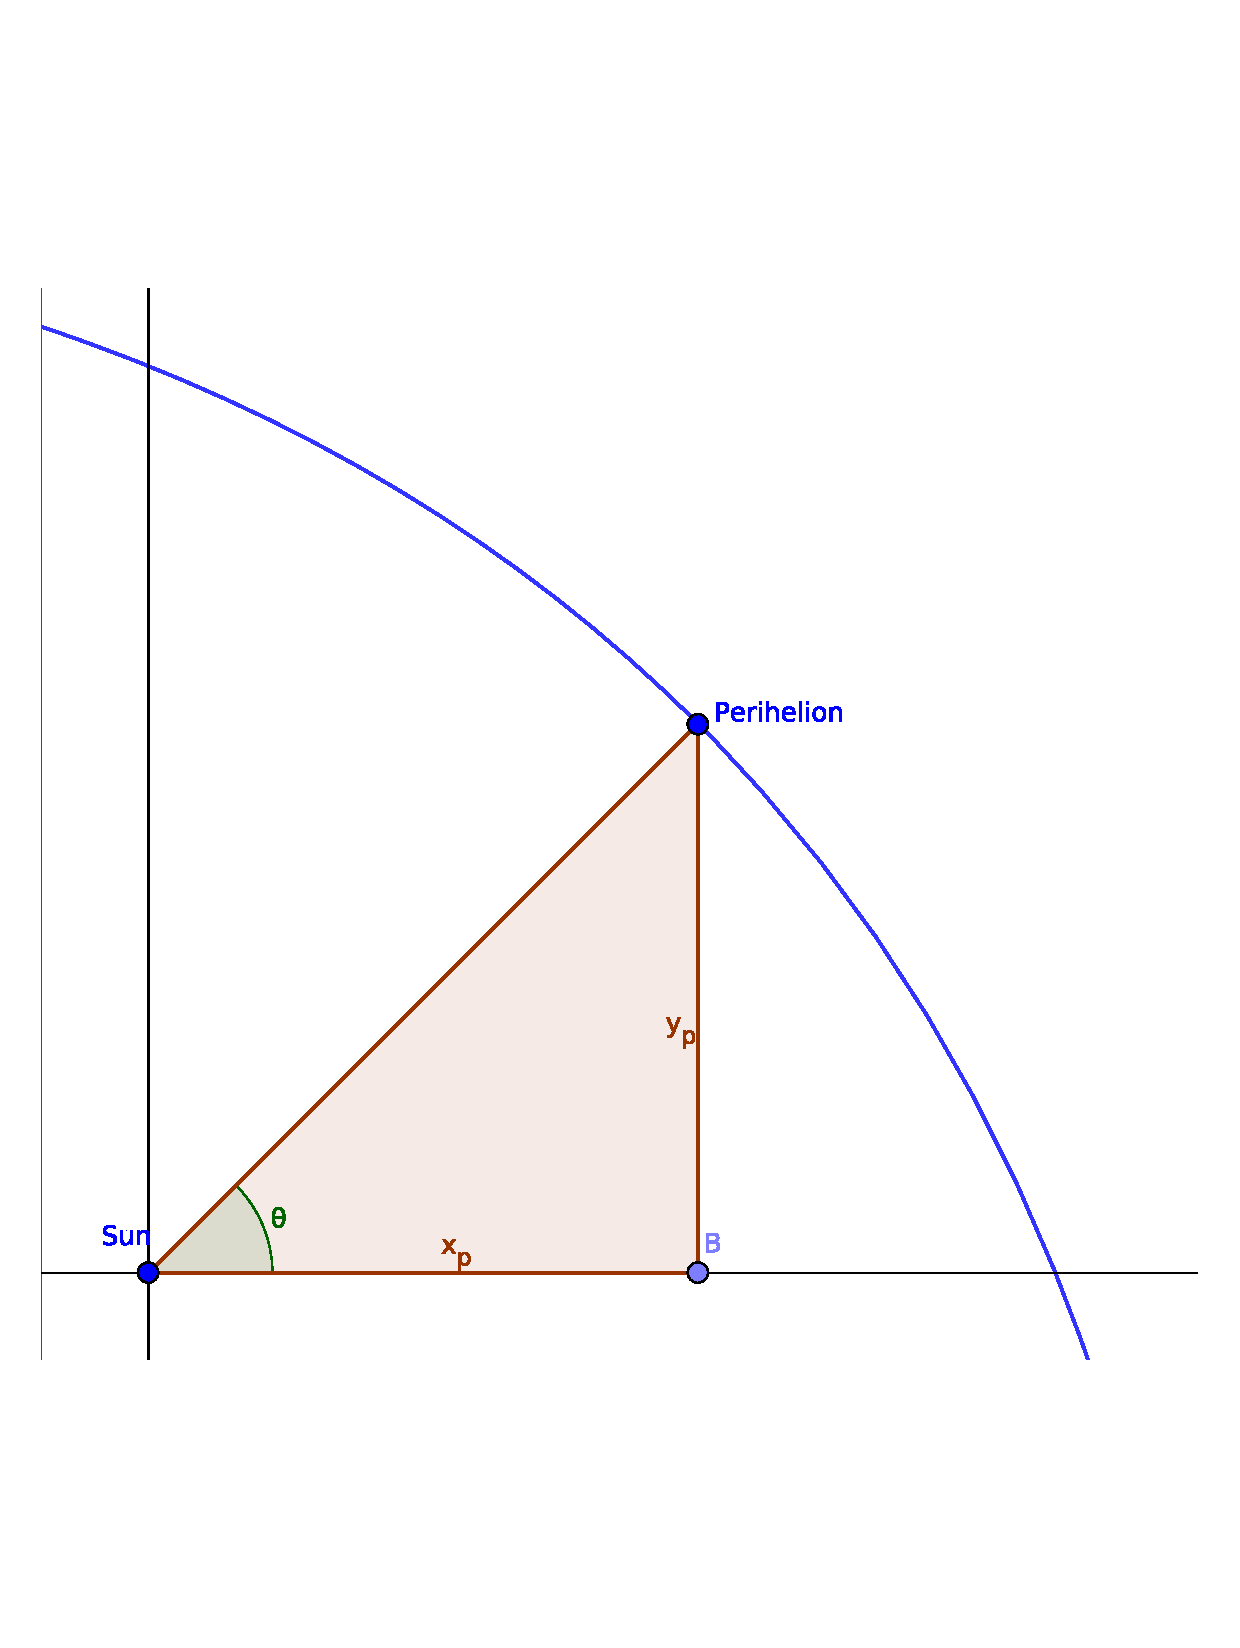
\includegraphics[width = 0.4\linewidth]{theory/bilder/figure.pdf}
	\caption{The figure shows the angle ($\theta$) and coordinates $(x_p,y_p)$ for the perihelion of Mercury. And with the formula $\tan \theta = \frac{opposite}{adjacent}$}
\end{figure}






\subsection{Numerical methods}

Equation (\ref{eq:acceleration_all_au}),initial conditions and the standard relations between position, velocity, acceleration determine the orbit of the planets. These equations are for x,y and z direction, written out you get a coupled set of differential equations. This set is near impossible to solve analytically. It might be impossible. We will use numerical methods to solve this set. More specifically we will use the Forward Euler method and the Velocity-Verlet method. A given $t_i$ is equal to $t_0 + ih$, where $h = (t_{0} + t_{n})/n $.













\subsubsection{Forward Euler}

Both methods use a Taylor polynomial approximation to solve the set of differential equation. The Forward Euler uses the first order Taylor polynomial. With $r'(t) = v(t)$ and $v'(t) = a(t)$ the Forward Euler method results in: 
 
\begin{align}
	&\vec{r_i}(t+h) \approx \vec{r_i}(t) + h \vec{v_i}(t)
	\\
	&\vec{v_i}(t+h) \approx \vec{v_i}(t) + h \vec{a_i}(t)
\end{align}

Discretized version. i is the object number and j is the time step:

\begin{align*}
	&\vec{r_{i,j+1}} \approx \vec{r_{i,j}} + h \vec{v}_{i,j}
	\\
	&\vec{v_{i,j+1}} \approx \vec{v_{i,j}} + h \vec{a}_{i,j}
\end{align*}

The error for a first order taylor polynomial goes as $\mathcal{O}(h^3)$ \cite{compphys}. This is the error for each step. The error is accumulated for each step and will therefore be proportional to h. 













\subsubsection{Velocity-Verlet}

You guessed it, this is the second order Taylor polynomial. As I said the Velocity-Verlet method is based on a Taylor polynomial approximation. And this is the second order. 

\begin{align}
	&\vec{r_i}(t+h) \approx \vec{r_i}(t) + h \vec{v_i}(t) + \frac{1}{2} h^2 a(t)
	\\
	&\vec{v_i}(t+h) \approx \vec{v_i}(t) + h \vec{a}(t) + \frac{1}{2} h^2 \vec{a}'(t)
	\label{eq:verlet}
\end{align}

Since we have no formula for the derivative of a, we use the approximation: 

\begin{align*}
	\vec{a}'(t) \approx \frac{\vec{a}(t+h) - \vec{a}(t)}{h}
\end{align*}

We simply update the position first. We keep the old acceleration and calculate the acceleration at the new position.  Using this and equation (\ref{eq:verlet}) we get: 

\begin{align*}
	&\vec{v_i}(t+h) \approx \vec{v_i}(t) + h \vec{a}(t) + \frac{1}{2} h(\vec{a}(t+h) - \vec{a}(t))
	\\
	&\vec{v_i}(t+h) \approx \vec{v_i}(t) + \frac{1}{2} h(\vec{a}(t+h) + \vec{a}(t))
\end{align*}

Discretized version. i is the object number and j is the time step:
\begin{align*}
	\\
	&\vec{r}_{i,j+1} \approx \vec{r}_{i,j} + h \vec{v}_{i,j} + \frac{1}{2} h^2 a_{i,j}
	\\
	&\vec{v}_{i,j+1} \approx \vec{v}_{i,j} +\frac{1}{2} h(\vec{a}_{i,j+1} + \vec{a}_{i,j})
\end{align*}


The error for a first order taylor polynomial goes as $\mathcal{O}(h^2)$ \cite{compphys}. This is the error for each step. The error is accumulated for each step and will thereby be proportional to $h^2$. This is one order of magnitude better, then the Forward Euler method. 




















\section{Method}
\subsection{Implementation of code}

The programs is writen in c++ and is object oriented. We found it natural to divide the project in to two classes and one main program. 
\\
\\
We made one class for the planets (\href{https://github.com/erikfsk/Project-3/blob/master/Project3/planet.cpp}{\textcolor{blue}{planet.cpp}} and \href{https://github.com/erikfsk/Project-3/blob/master/Project3/planet.h}{\textcolor{blue}{planet.h}}). This class contain variables for the position, velocity, mass for the specific planet and a specific filename. The class has methods for updating position, velocity and acceleration as outlined in section \ref{sec:theory}. In addition, methods for writing to a file was implemented. 
\\
\\
The second class is for the solarsystem (\href{https://github.com/erikfsk/Project-3/blob/master/Project3/solarsystem.cpp}{\textcolor{blue}{solarsystem.cpp}} and \href{https://github.com/erikfsk/Project-3/blob/master/Project3/solarsystem.h}{\textcolor{blue}{solsystem.h}}). The solar system contain a list with all the planets and has methods to make the planets move and interact to each other. You can look at the solar system as a class with for-loops for the planets. 
\\
\\
The \href{https://github.com/erikfsk/Project-3/blob/master/Project3/main.cpp}{\textcolor{blue}{main.cpp}} program is where all the inputs to the solar system is given. Here all the initial conditions for the planets are stated and organized for proper input to the solarsystem class.
\\
\\
All these programs are combined with \href{https://github.com/erikfsk/Project-3/blob/master/Project3/makefile}{\textcolor{blue}{makefile}}. When this is done the \href{https://github.com/erikfsk/Project-3/blob/master/Project3/solsys.exe}{\textcolor{blue}{solsys.exe}} will be made. It takes in three arguments. The first argument is the number of planets that you would like to simulate. This is a preset list of the bodies in the solarsystem. Where the Sun is the first element, Earth is the second and Jupiter is the third. After that they ascend based on orbital radius. The second argument is the end time for the simulation measured in years from now. The start time is set to 19th of october 2017. This is the time that the intial values were obtained from \href{https://ssd.jpl.nasa.gov/horizons.cgi#top}{\textcolor{blue}{NASA}}. Finally the third argument is the number of steps, n. 
\\
\\
Finally, in our github repository there are directories where earlier versions can be found. For instance the 
\href{https://github.com/erikfsk/Project-3/tree/master/Project3/}{\textcolor{blue}{Project3}} directory is for where all the code is centered. In this directory there are many directories with different results files and python scripts for making figures. There are also a coupled of other main.cpp variants. These are for different assignments in this project. It should be pretty self ex<planet>ory. 


\subsection{FLOPs for the algorithms}\label{sec:flops}

The counting of the FLOPs are in section \ref{sec:appendix} Appendix. There we show sudo-code. For each line of code there is a corresponding comment that counts flops. For each method there is a header comment explaining what method and algorithm it represents. After each method there is a final comment with total FLOPs.
\\
\\
Common for both algorithms are calculation of the acceleration. The acceleration itself is 19 FLOPs. But for both algorithm this is called $n(n-1)$ times. After that the Forward Euler method calls functions to set position and velocity. This is done for all the planets. And for each planet it costs 6 FLOPs for the position and 6 more for the velocity. This gives a total of:

\begin{align*}
	19n(n-1) + 12n = 19n^2 - 7n
\end{align*}

For the Verlet-Velocity it is 21 FLOPs for the position and 12 FLOPs for the velocity (nothing is precalculated). This is of course done for all the planets and gives us: 

\begin{align*}
	19n(n-1) + 33n = 19n^2 + 14n
\end{align*}
%((19*(9^2) + 14*9)- (19*(9^2) - 7*9)) /(19*(9^2) -7*9)
So, this means that for 9 planets the verlet method has about 13 \% more FLOPs, which is not much considering that the majority of run time is not spent on these calculations but rather on writing to file, getting variables etc. As a result, a minimal run time discrepancy is expected





























\section{Result \& Discussion}











\subsection{Earth-Sun system}








\subsubsection{Stability}

\begin{figure}[H]
    \centering
    \begin{subfigure}{0.5\textwidth}
        \centering
        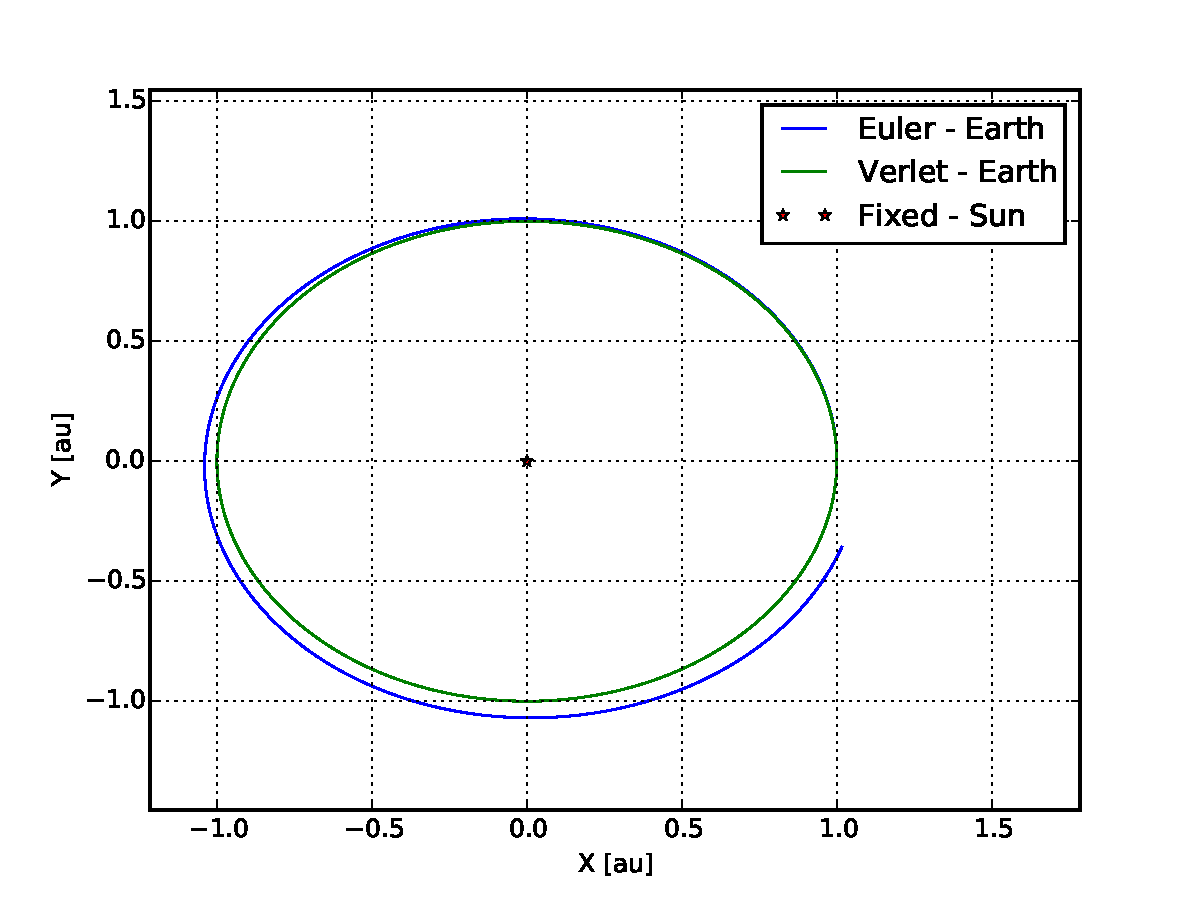
\includegraphics[width=\linewidth]{result/bilder/earth-sun.pdf}
    	\caption{}
    \end{subfigure}%
    ~ 
    \begin{subfigure}{0.5\textwidth}
        \centering
        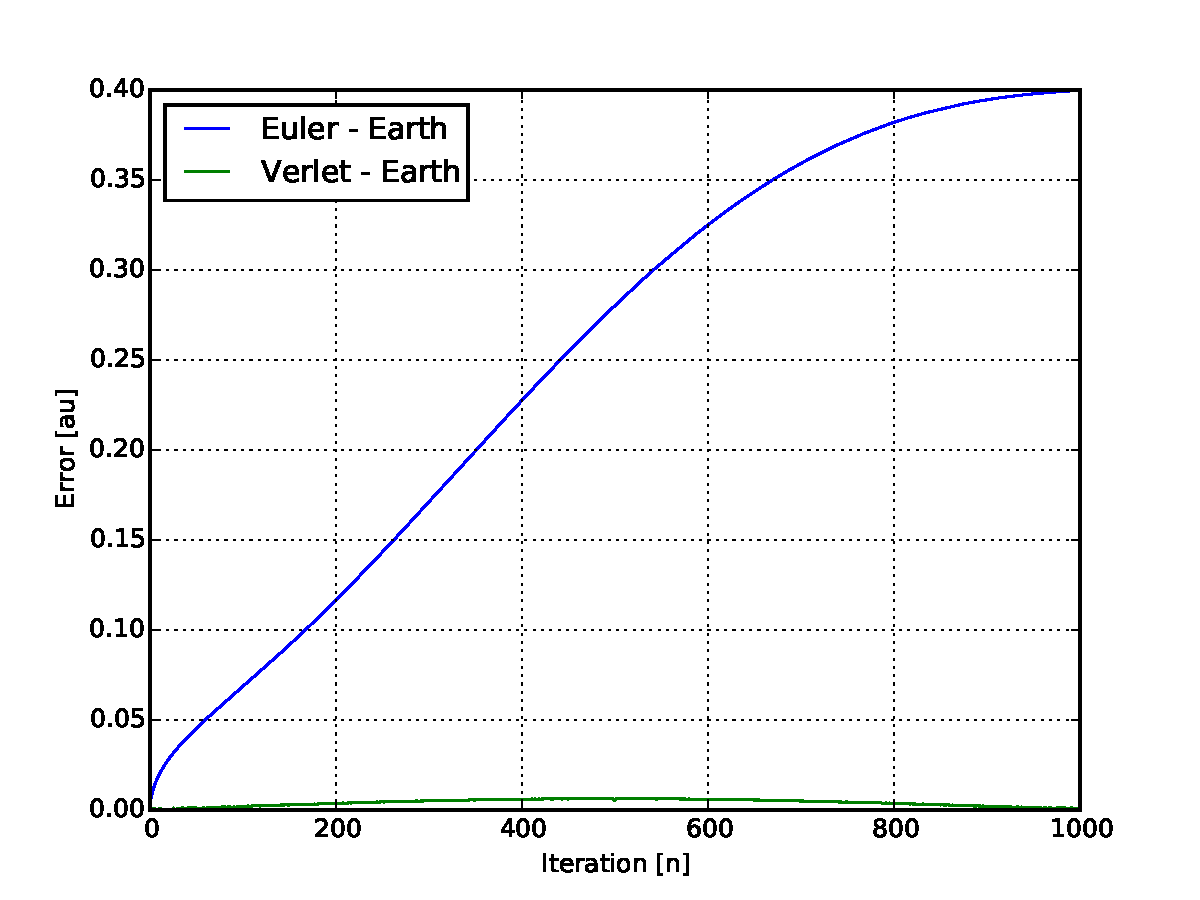
\includegraphics[width=\linewidth]{result/bilder/earth-sun-error.pdf}
        \caption{}
    \end{subfigure}
    \caption{a) shows the orbit of earth around the sun. The intial velocity is set to $2\pi$ in y direction and the start position to 1 au in x direction. b) shows how the error develops. The intial values should give a perfect circular motion. So the error is calculated by $r_i - r_{0}$. It is apparent that the Verlet-Velocity method is a better approximation. This simulation was with 1000 points with the end time of 1 year. Both simulations was produced by \href{https://github.com/erikfsk/Project-3/tree/master/Project3/earth-sun-standard-results}{\textcolor{blue}{plot\_earth\_sun.py}}}
    \label{fig:earth-sun}
\end{figure}


\begin{center}
\label{table:euler-verlet-time}
\captionof{table}{Time table for the different algorithms. The algorithms use nearly the same time. This is not a shocker since the number of FLOPs for the algorithms are similar, see section (\ref{sec:flops}). Note: this is only the result from one test, but several was done. Both algorithms were very close and it seems to be random which is fastest.
\\}
\begin{tabularx}{\textwidth}{c c c c c c c c}
    \hline 
    \hline 
    n & Forward-Euler & Verlet-Velocity &  fastest &&&& $\frac{slowest}{fastest}$\\ 
    \hline
    10 & 0.000136 & 0.000148 & Euler &&&&   1.08823529412   \\ 
    100 & 0.000208 & 0.000179 & Verlet &&&&   1.16201117318   \\ 
    1000 & 0.000392 & 0.000389 & Verlet &&&&  1.00771208226   \\ 
    10000 & 0.002427 & 0.002426 & Verlet &&&&   1.00041220115  \\ 
    100000 & 0.022931 & 0.022293 & Verlet &&&&   1.02861884897   \\ 
    1000000 & 0.167022 & 0.175944 & Euler &&&&   1.05341811258  \\ 
    10000000 & 1.58721 & 1.52666 & Verlet &&&&   1.03966174525  \\ 
    100000000 & 15.1786 & 15.1176 & Verlet &&&&   1.00403503202  \\ 
    \hline
\end{tabularx}
\end{center}














\subsubsection{Conserved quantities}

All the figures in this section was made from the data and python script in the directory \href{https://github.com/erikfsk/Project-3/tree/master/Project3/conserved-values}{\textcolor{blue}{conserved-values}}.

\begin{figure}[H]
    \centering
    \begin{subfigure}{0.5\textwidth}
        \centering
        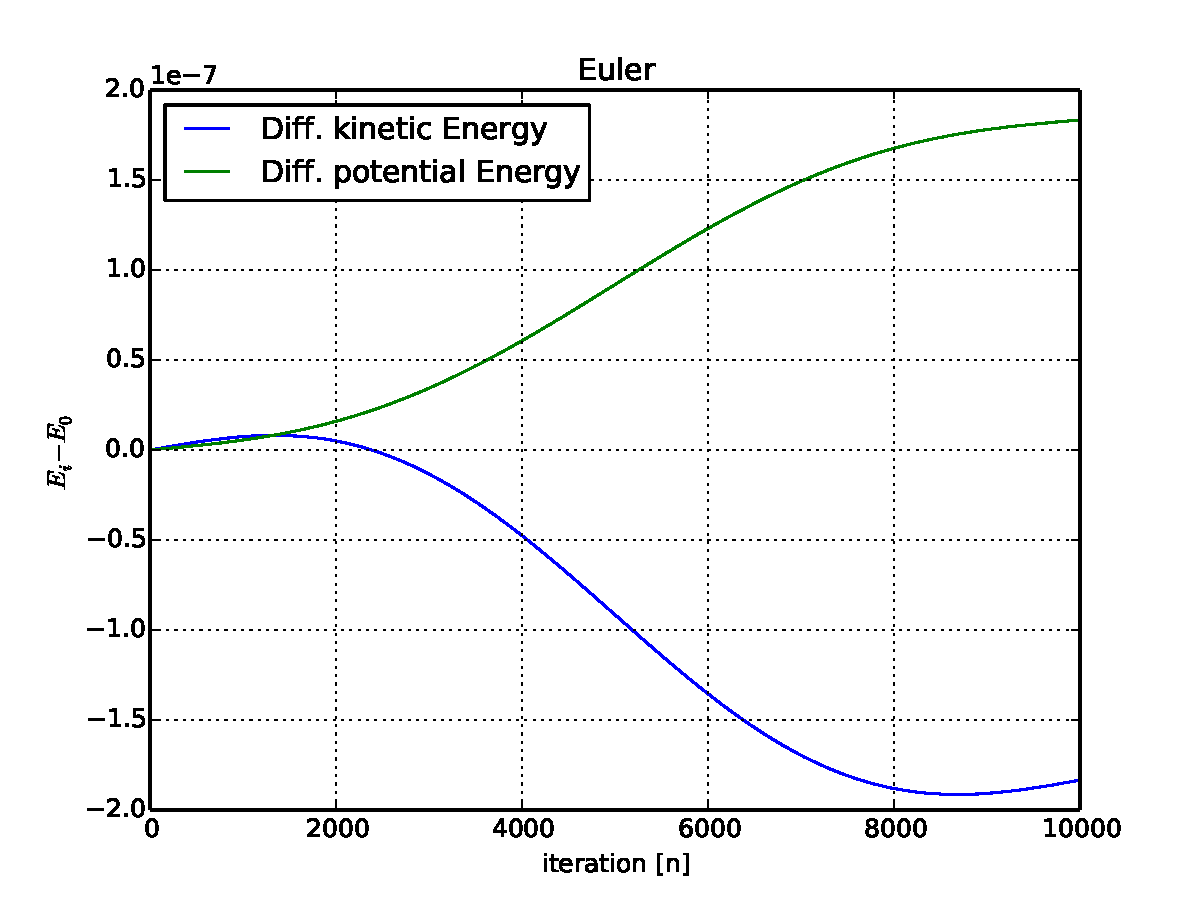
\includegraphics[width=\linewidth]{result/bilder/kin-pot-euler.pdf}
    	\caption{}
    \end{subfigure}%
    ~ 
    \begin{subfigure}{0.5\textwidth}
        \centering
        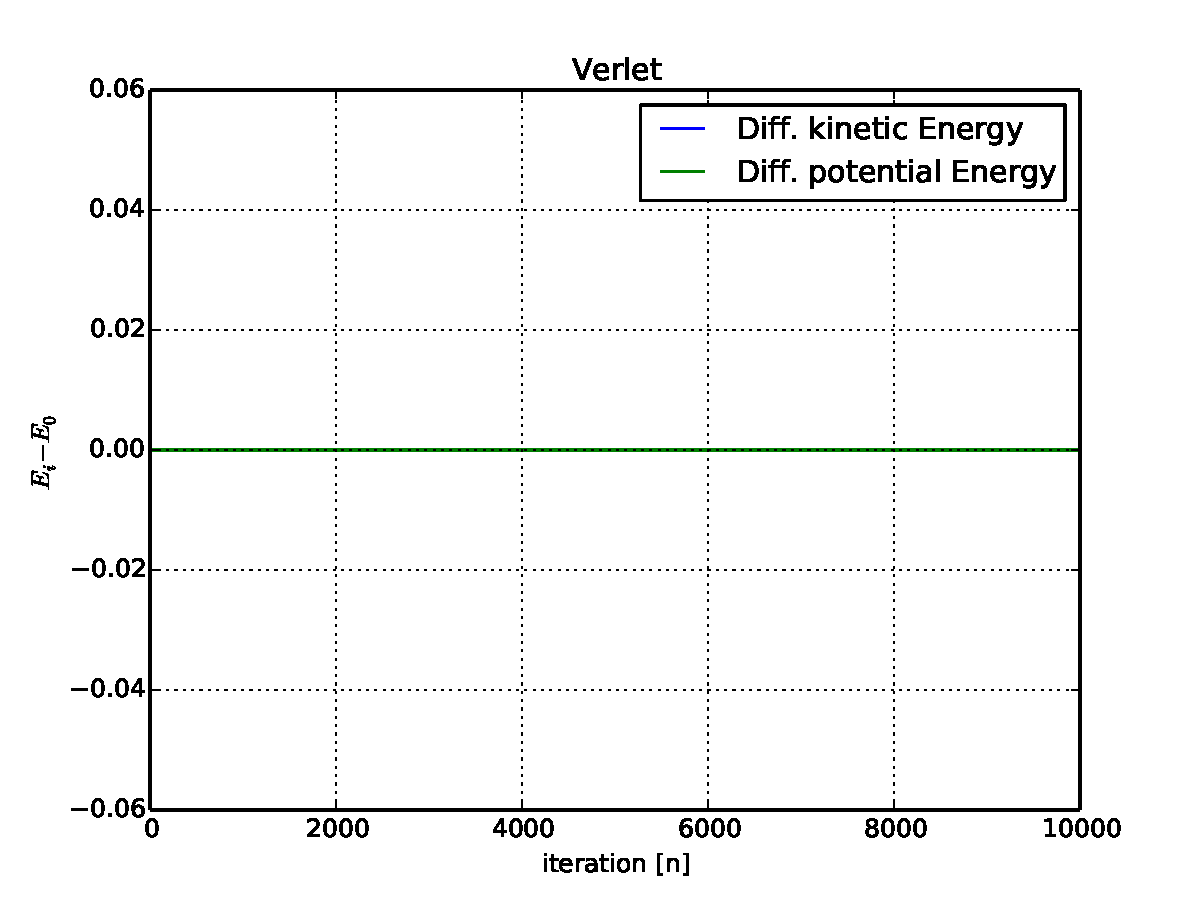
\includegraphics[width=\linewidth]{result/bilder/kin-pot-verlet.pdf}
        \caption{}
    \end{subfigure}
    \caption{The graphs show the change in kinetic and potential energies compared to their initial values a) is the Forward Euler method and b) is the Verlet-Velocity method.}
    \label{fig:conserved-energy}
\end{figure}

 As expected the energies are not conserved in the Forward Euler method, but is conserved in the Verlet-Velocity.



\begin{figure}[H]
    \centering
    \begin{subfigure}{0.5\textwidth}
        \centering
        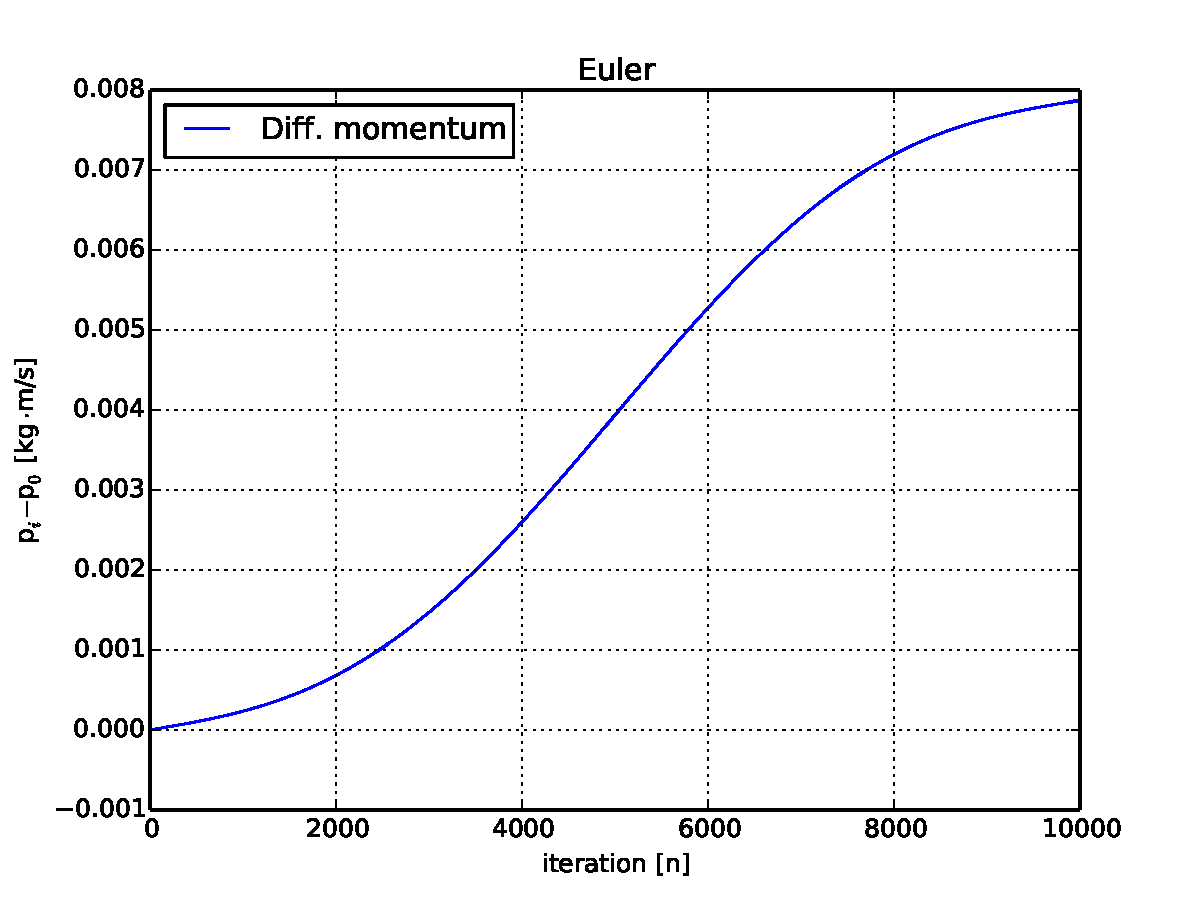
\includegraphics[width=\linewidth]{result/bilder/momentum-euler.pdf}
    	\caption{}
    \end{subfigure}%
    ~ 
    \begin{subfigure}{0.5\textwidth}
        \centering
        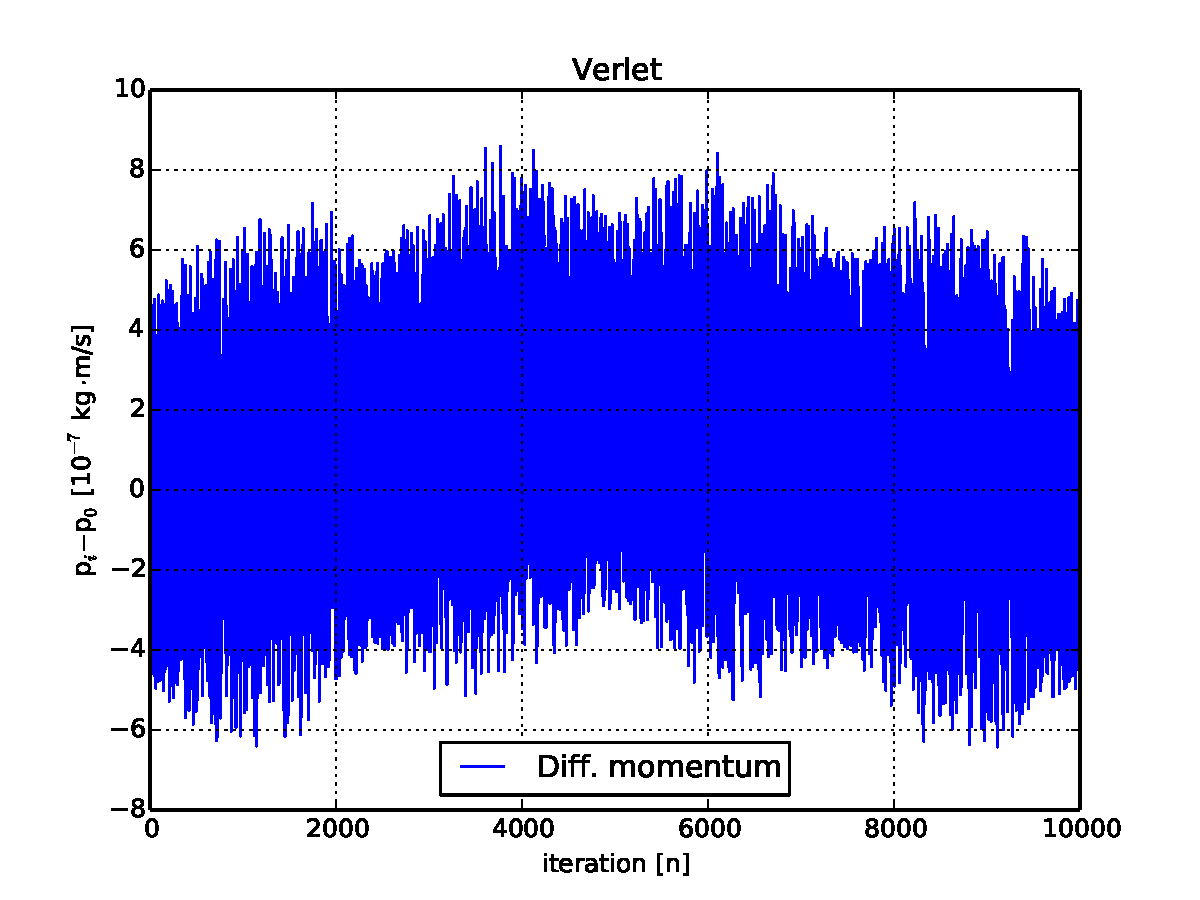
\includegraphics[width=\linewidth]{result/bilder/momentum-verlet.pdf}
        \caption{}
    \end{subfigure}
    \caption{Both graphs are of the momentum and how they differ from their intial values. a) is the Forward Euler method and b) is the Verlet-Velocity method.
    }
    \label{fig:conserved-momentum}
\end{figure}

 It should come as no suprise that momentum is not conserved for the Forward Euler method as the kinetic energy was not conserved. Once again the Verlet-velocity method conserves the quantity. 



\begin{figure}[H]
    \centering
    \begin{subfigure}{0.5\textwidth}
        \centering
        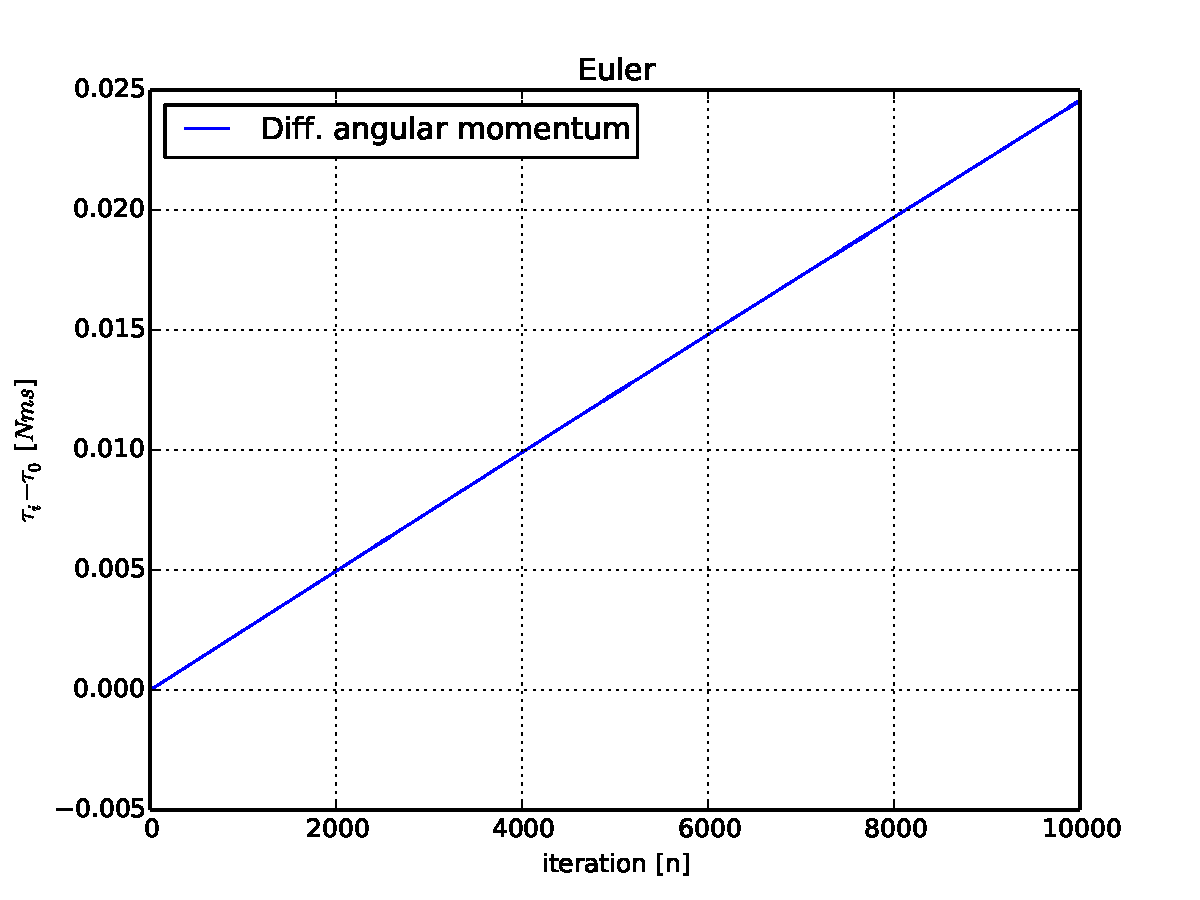
\includegraphics[width=\linewidth]{result/bilder/ang-momentum-euler.pdf}
        \caption{}
    \end{subfigure}%
    ~ 
    \begin{subfigure}{0.5\textwidth}
        \centering
        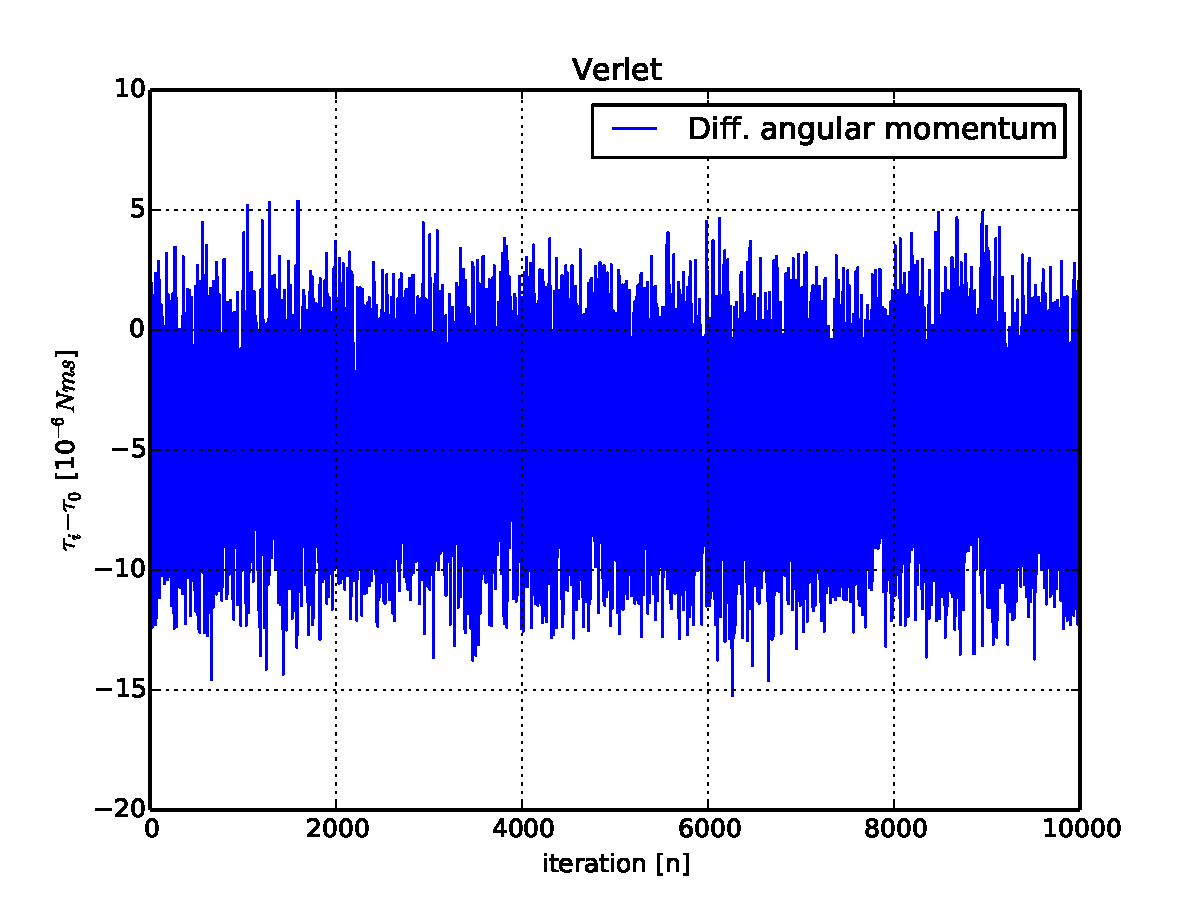
\includegraphics[width=\linewidth]{result/bilder/ang-momentum-verlet.pdf}
        \caption{}
    \end{subfigure}
    \caption{Both figures are graphs of the angular momentum and how they differ from their intial values. a) is the Forward Euler method and b) is the Verlet-Velocity method. 
    }
    \label{fig:conserved-ang}
\end{figure}

Forward Euler is once again not capable of conserving the value, but luckily for us the Verlet-Velocity method is. 













\subsubsection{Escape velocity}

The assignment was to find the escape velocity for the earth by trial and error. Fortunate for us that we know some math and can calculate it. See section \ref{sec:escape-velocity} for this. In practice this meant we started guessing "randomly" (winking Face emoji) before tuning the initial conditions to find the escape velocity. Figure (\ref{fig:escape-velocity-low}) a) shows these guesses where we can see that the velocities of around 8.8 au/yr causes the planet to shoot out and never return. 
The algorithms only runs for 15 years and will thereby not see the 8.8 au/year return to orbit even though it should. The plots were made by the data and python scripts in the directory \href{https://github.com/erikfsk/Project-3/tree/master/Project3/escape-velocity}{\textcolor{blue}{escape-velocity}}.

\begin{figure}[H]
    \centering
    \begin{subfigure}{0.5\textwidth}
        \centering
        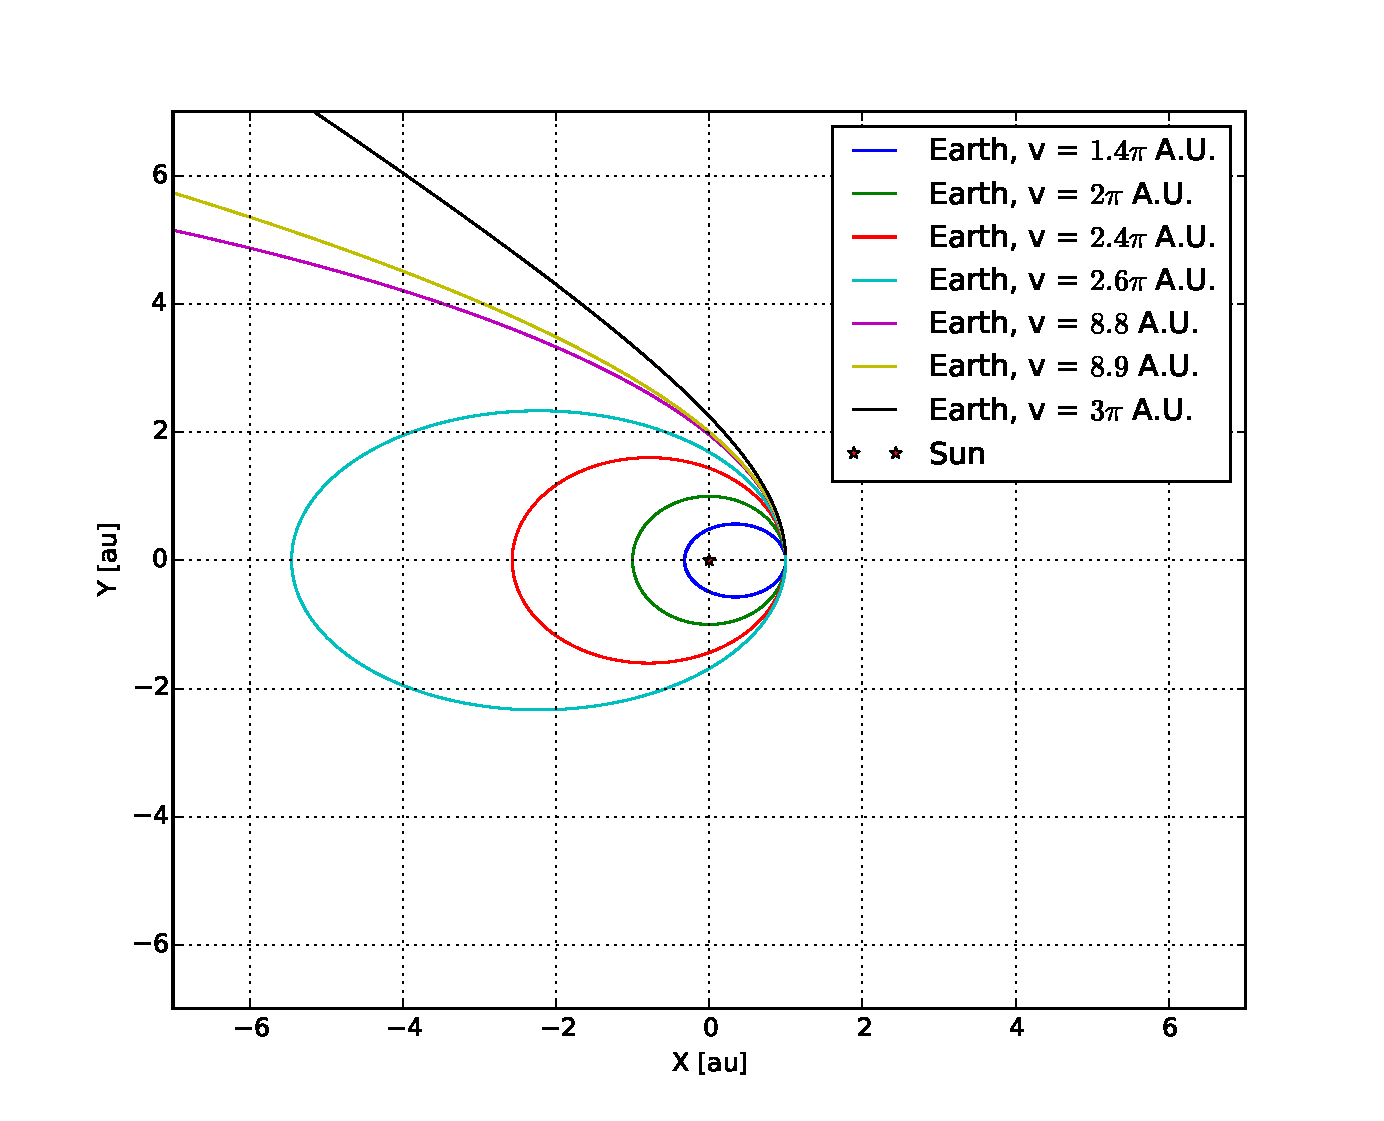
\includegraphics[width=\linewidth]{result/bilder/escape-velocity.pdf}
    	\caption{}
    \end{subfigure}%
    ~ 
    \begin{subfigure}{0.5\textwidth}
        \centering
        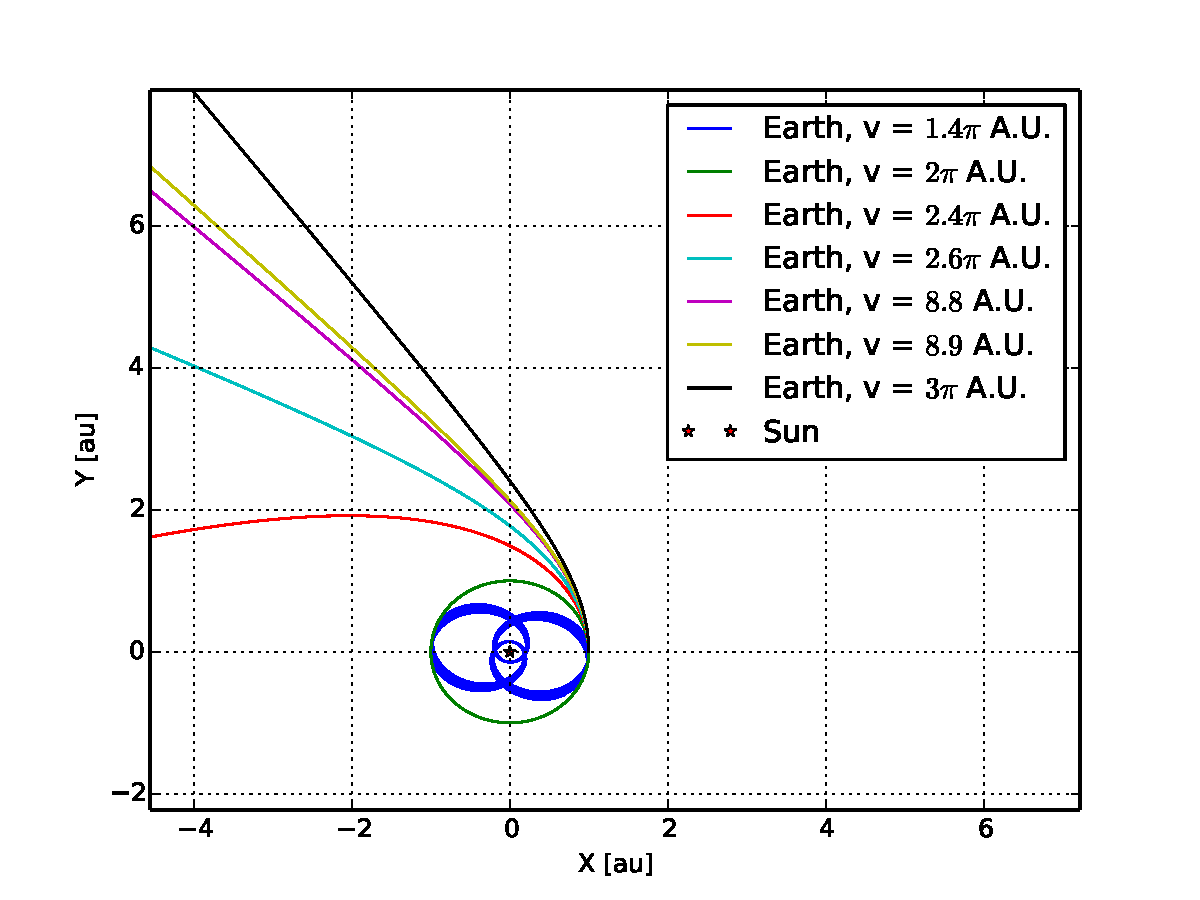
\includegraphics[width=\linewidth]{result/bilder/escape-velocity-r25.pdf}
        \caption{}
    \end{subfigure}
    \caption{a) Shows how the orbits of earths with different initial velocity develops. b) Shows the same as a) but this time the dependency of r in the denominator in equation (\ref{eq:newton}) is set to 3.5.}
    \label{fig:escape-velocity-low}
\end{figure}



\begin{figure}[H]
    \centering
    \begin{subfigure}{0.5\textwidth}
        \centering
        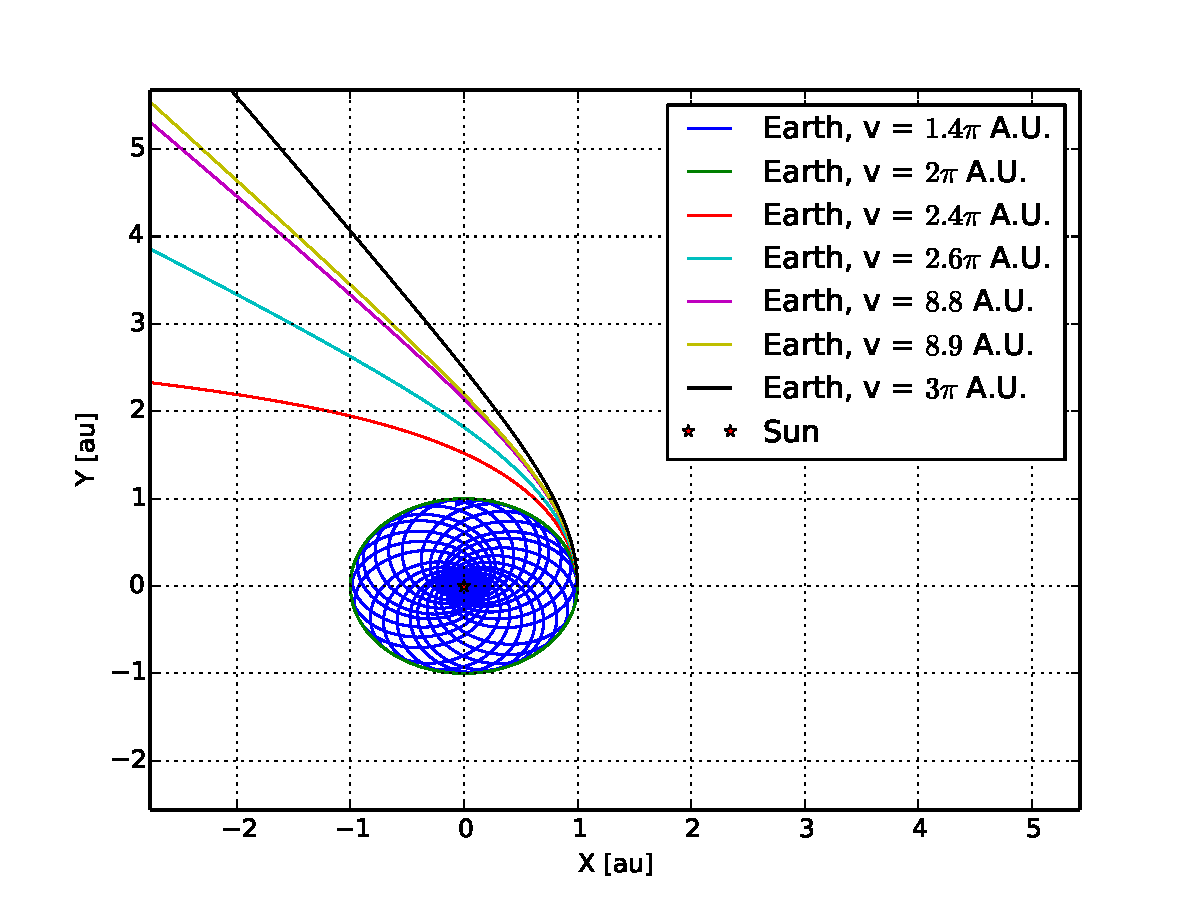
\includegraphics[width=\linewidth]{result/bilder/escape-velocity-r275.pdf}
    	\caption{}
    \end{subfigure}%
    ~ 
    \begin{subfigure}{0.5\textwidth}
        \centering
        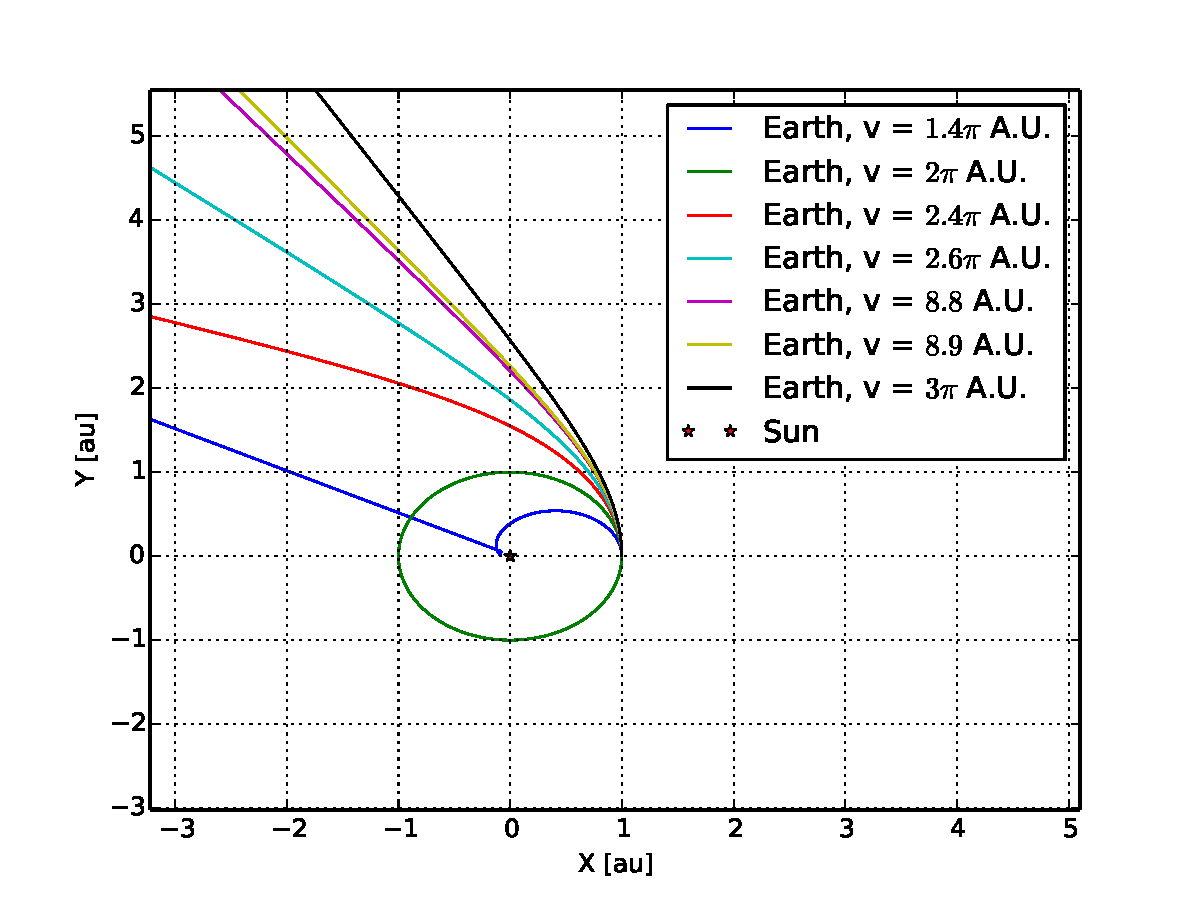
\includegraphics[width=\linewidth]{result/bilder/escape-velocity-r3.pdf}
        \caption{}
    \end{subfigure}
    \caption{a) Shows the same as figure (\ref{fig:escape-velocity-low}) but this time the dependency of r in the denominator in equation (\ref{eq:newton}) is set to 3.75. b) again shows the same as a) but now with the denominator set to 4.}
    \label{fig:escape-velocity-high}
\end{figure}


We are extremly lucky for living in a universe with a radius dependency of 2, but then again we probably would not exist if the dependency was different. All the other dependencies are very unstable for even the slightest change in velocity from the circular orbit velocity.


















\subsection{Three body system}

All the figures in this section has been made from the directory \href{https://github.com/erikfsk/Project-3/tree/master/Project3/mass%20jupitur}{\textcolor{blue}{mass jupitur}}. In this directory there are different directories for the r dependency and a python script to generate graphs. The effect of varying Jupiters mass was quite striking, as we saw in the simulations. Four different masses with factors of 10, 100, 1000 and 1100 was compared and can be seen in the plots below.

\subsubsection{Fixed mass for Jupitur}

For a simulation with Jupiters original mass $10^5$ points over 15 years is sufficient to calculate the orbits of the planets. Figure (\ref{fig:three-body}) is quite smooth and one should not expect to get any major change in the result even with many more points per year. 

\begin{figure}[H]
    \centering
    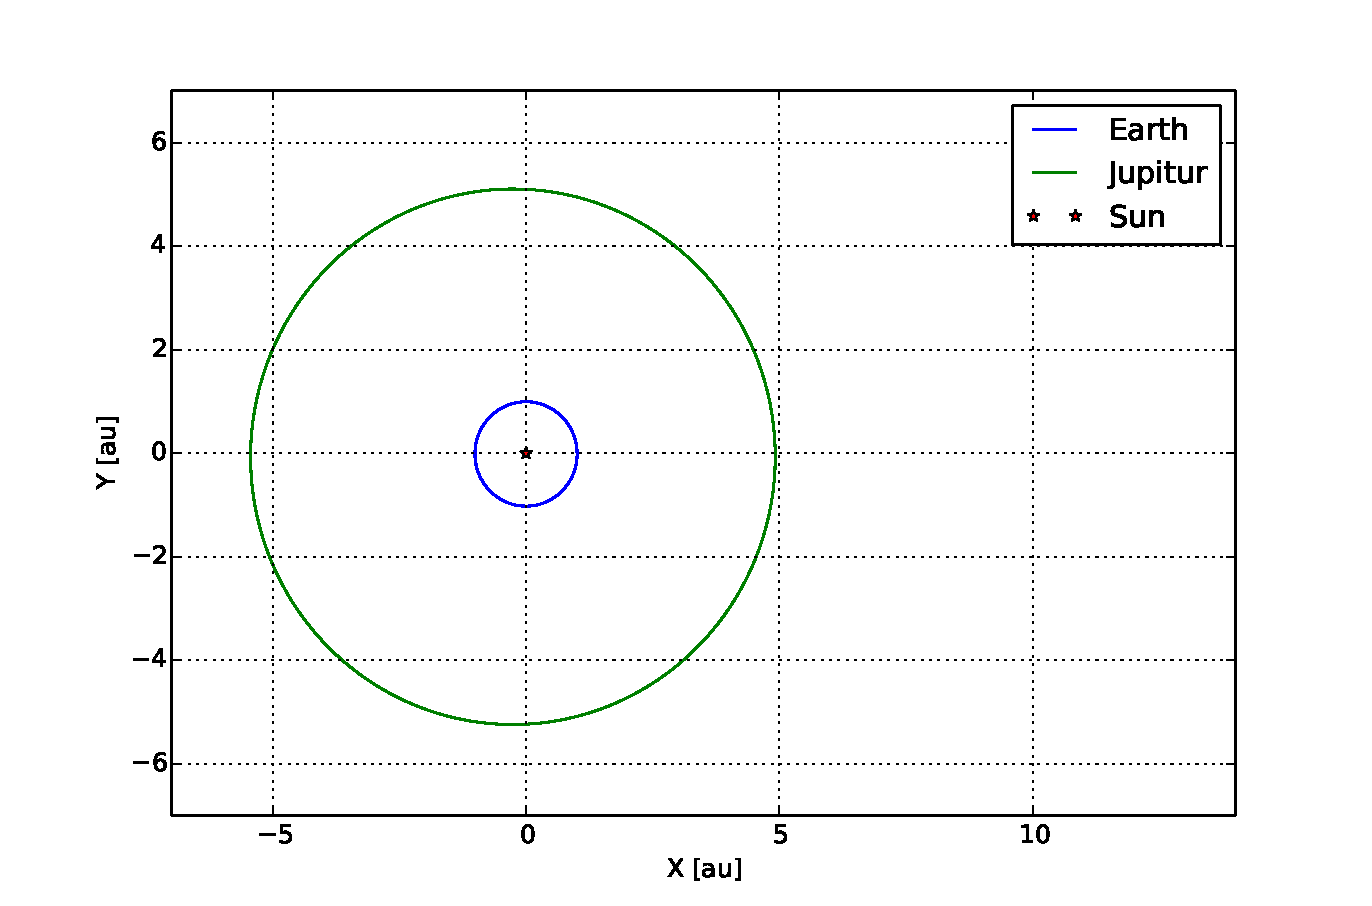
\includegraphics[width=\linewidth]{result/bilder/jupitur-mass.pdf}
    \caption{Plot of the three body system with Earth, Jupitur and the sun. n = 100000 over 15 years. The graph is discussed in the paragraph above. }
    \label{fig:three-body}
\end{figure}


\subsubsection{Varying mass for Jupiter}

For varying mass it is mostly the same as for the original mass. For the mass multiplied with 10 and 100 the orbit is normal with some slight changes and one should not expect any major differences with higher amount of points per year. For the biggest masses the results vary much more on the number of steps per year. We found that a couple of hundred thousand steps in total gave a good approximation. A bit higher step count makes earth disappear and a way bigger step count makes the earth come back to orbit like shown below. This is basicly the best of both worlds. The graphs has a relatively low amount of points, making it easier for the python plot, and has a pretty good approximation.

\begin{figure}[H]
    \centering
    \begin{subfigure}{0.5\textwidth}
        \centering
        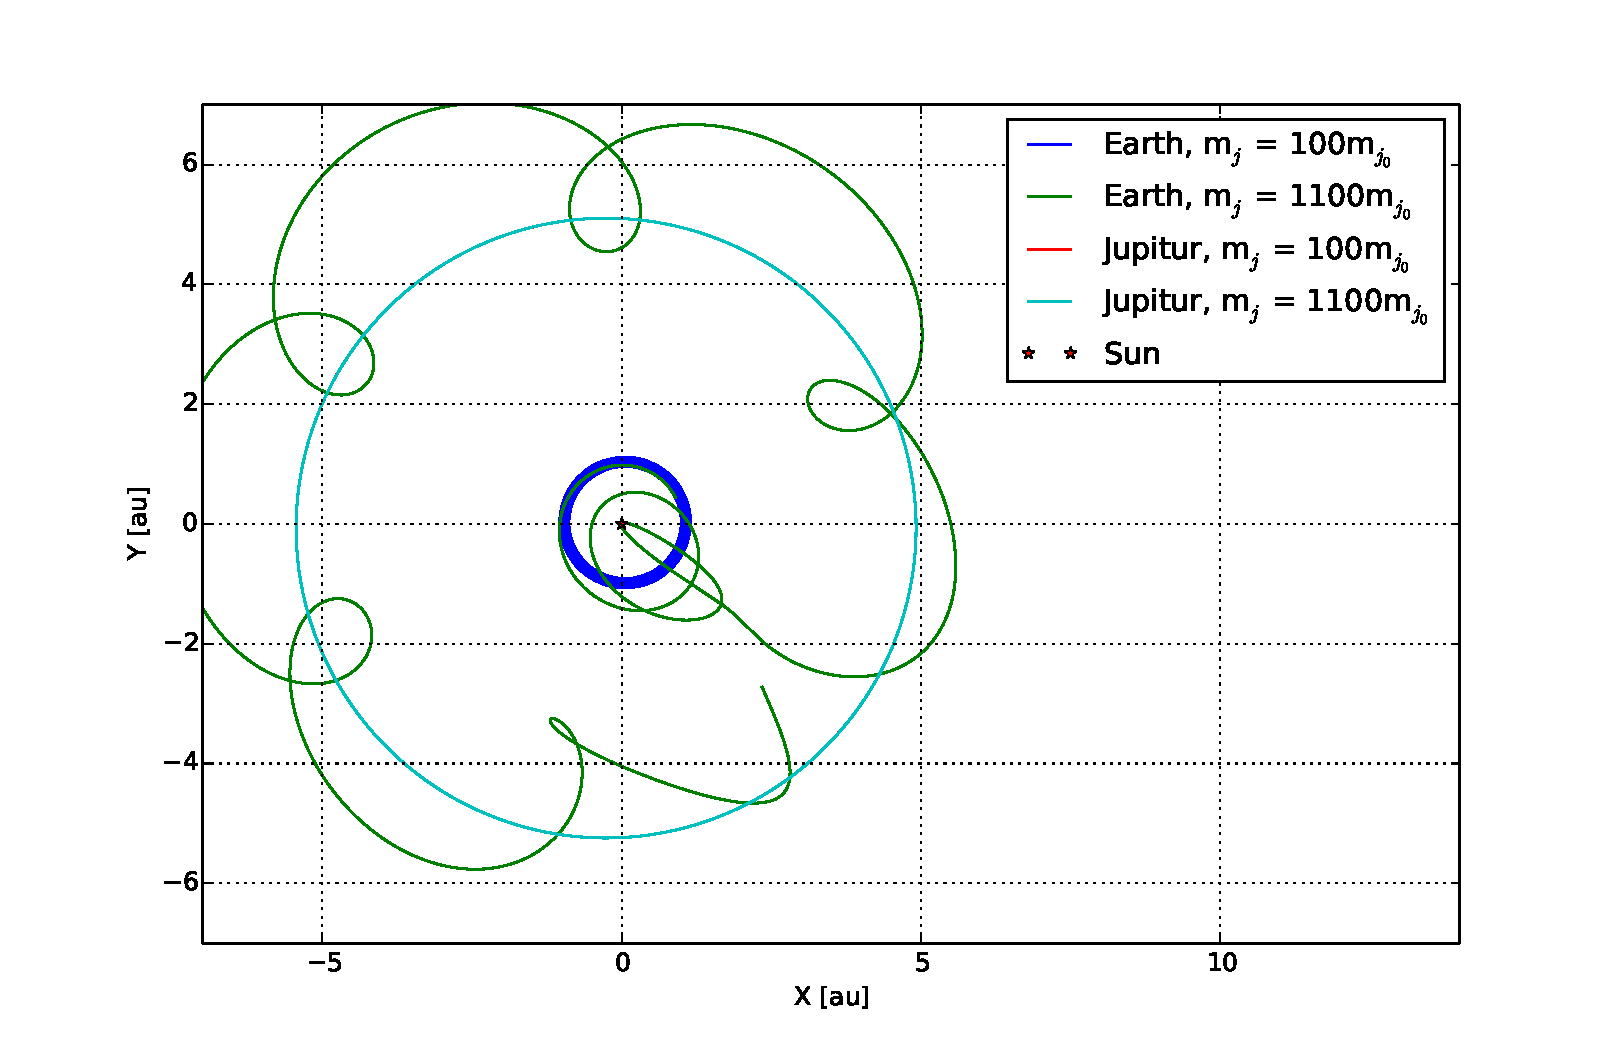
\includegraphics[width=\linewidth]{result/bilder/jupitur-mass-three.pdf}
    	\caption{}
    \end{subfigure}%
    ~ 
    \begin{subfigure}{0.5\textwidth}
        \centering
        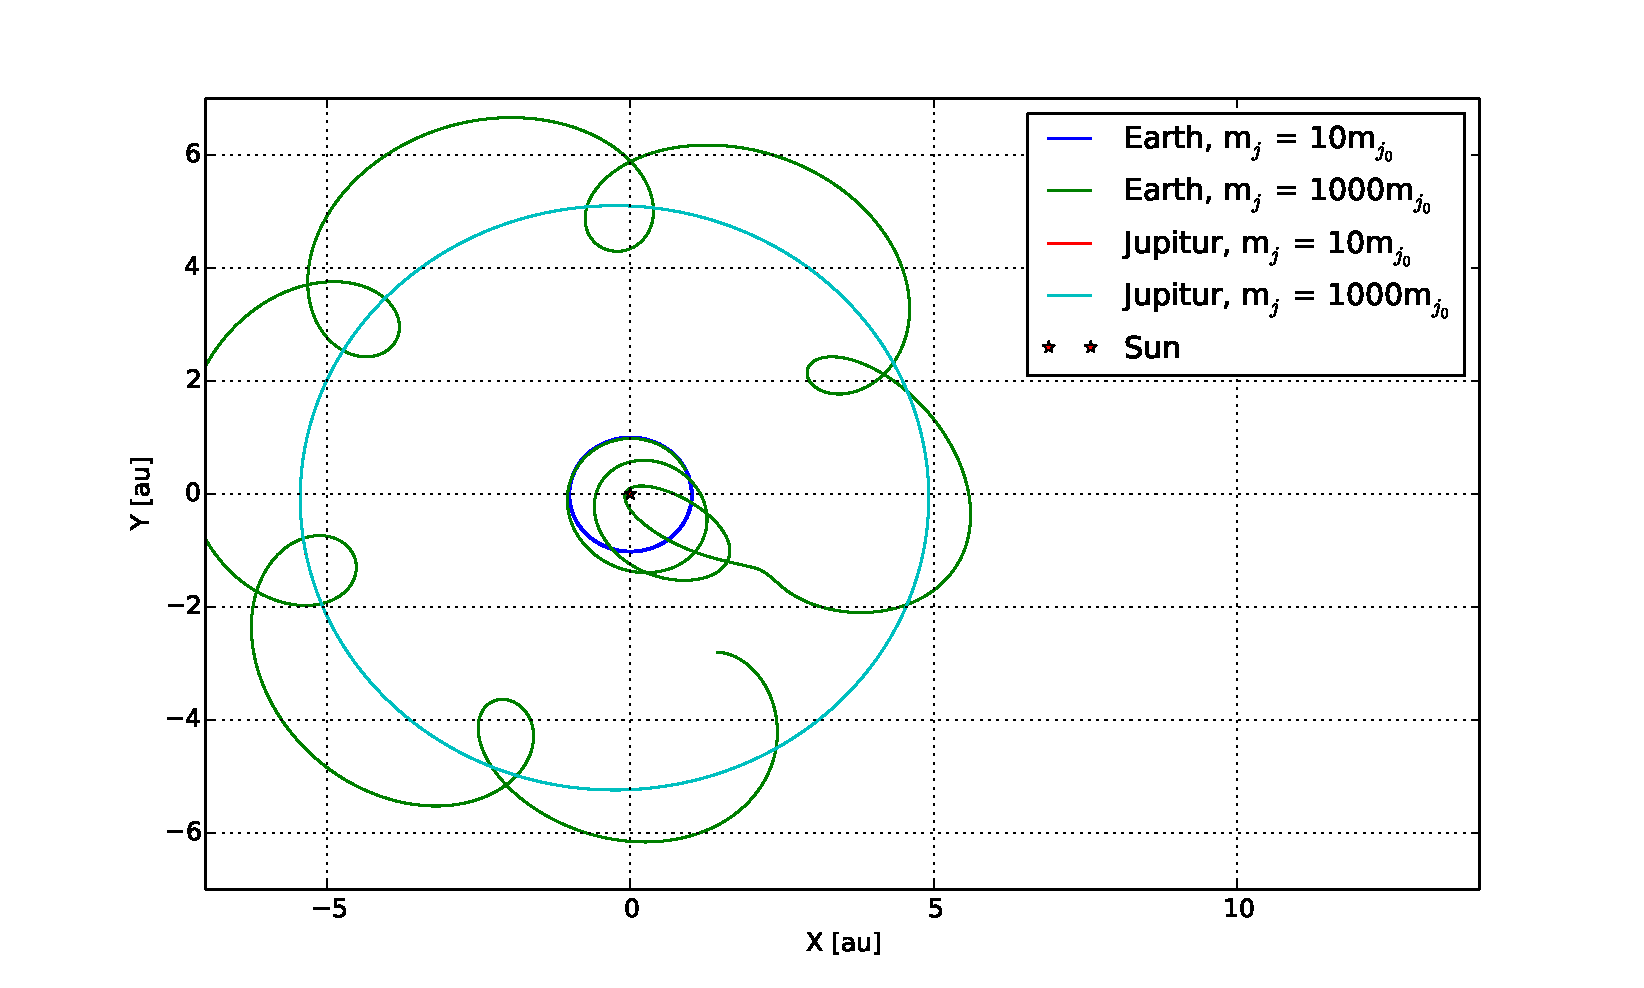
\includegraphics[width=\linewidth]{result/bilder/jupitur-mass-two.pdf}
        \caption{}
    \end{subfigure}
    \caption{Both plots has the sun as a fixed point. n = 100000 over 15 years. What the graphs represent is discussed above and legend should be pretty self explanatory.}
    \label{fig:three-body-varying}
\end{figure}











\subsection{Solar system}

All the figures in this section was made from the results and python scripts in the directory \href{https://github.com/erikfsk/Project-3/tree/master/Project3/full-solarsystem}{\textcolor{blue}{full-solarsystem}}.

\subsubsection{Three planets and all moving}

\begin{figure}[H]
    \centering
    \begin{subfigure}{0.5\textwidth}
        \centering
        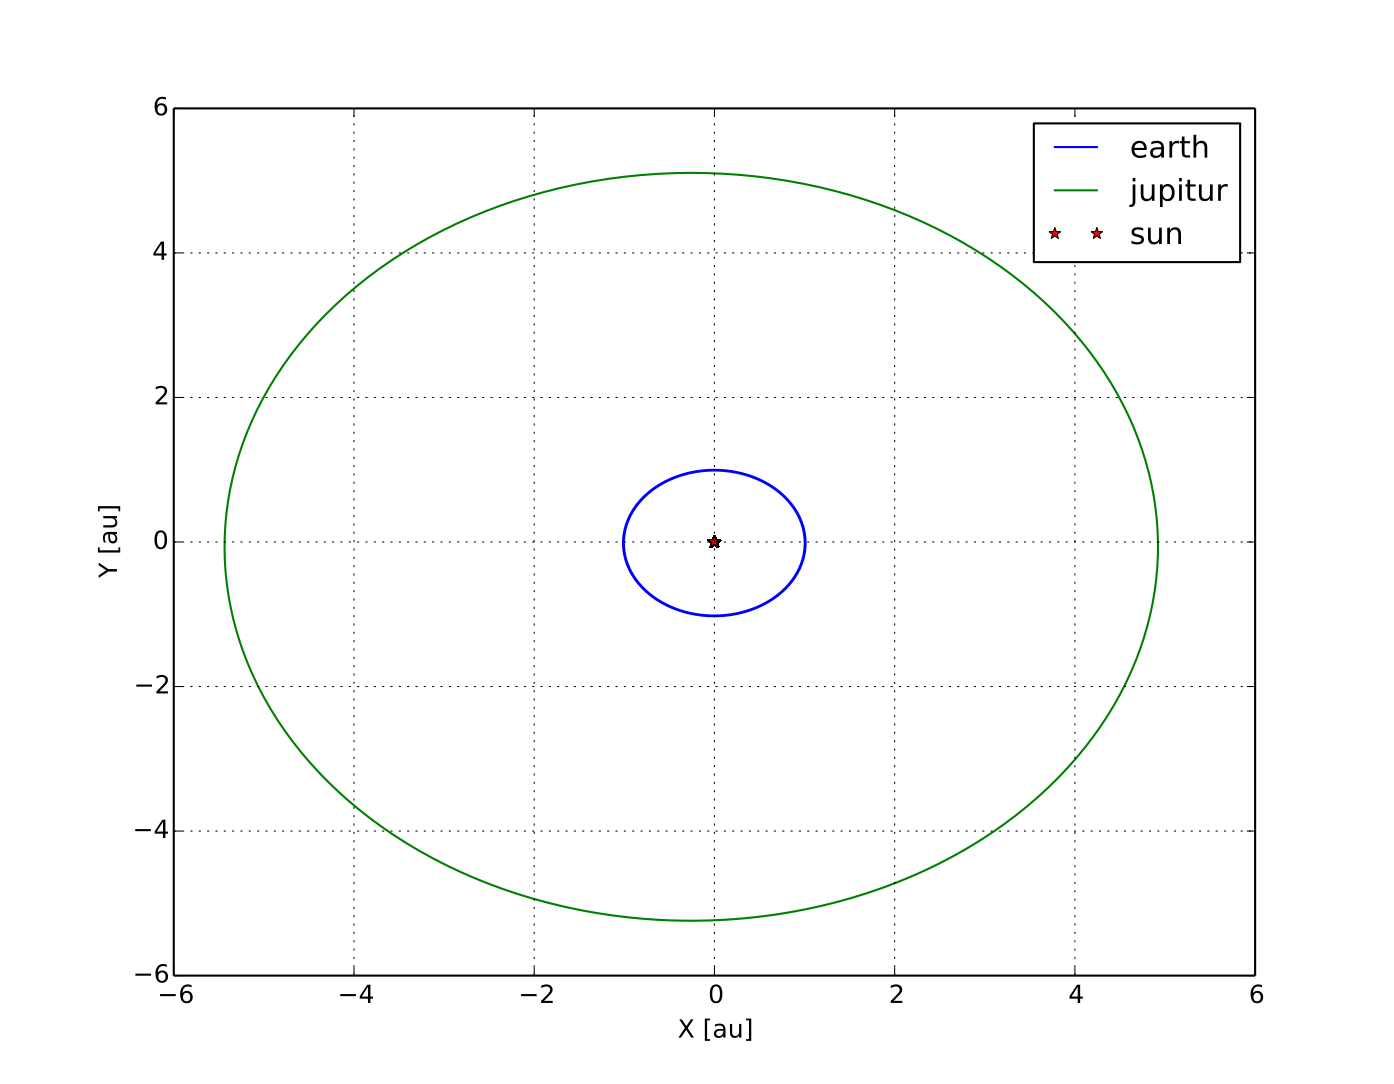
\includegraphics[width=\linewidth]{result/bilder/all-moving-jupitur.png}
        \caption{}
    \end{subfigure}%
    ~ 
    \begin{subfigure}{0.5\textwidth}
        \centering
        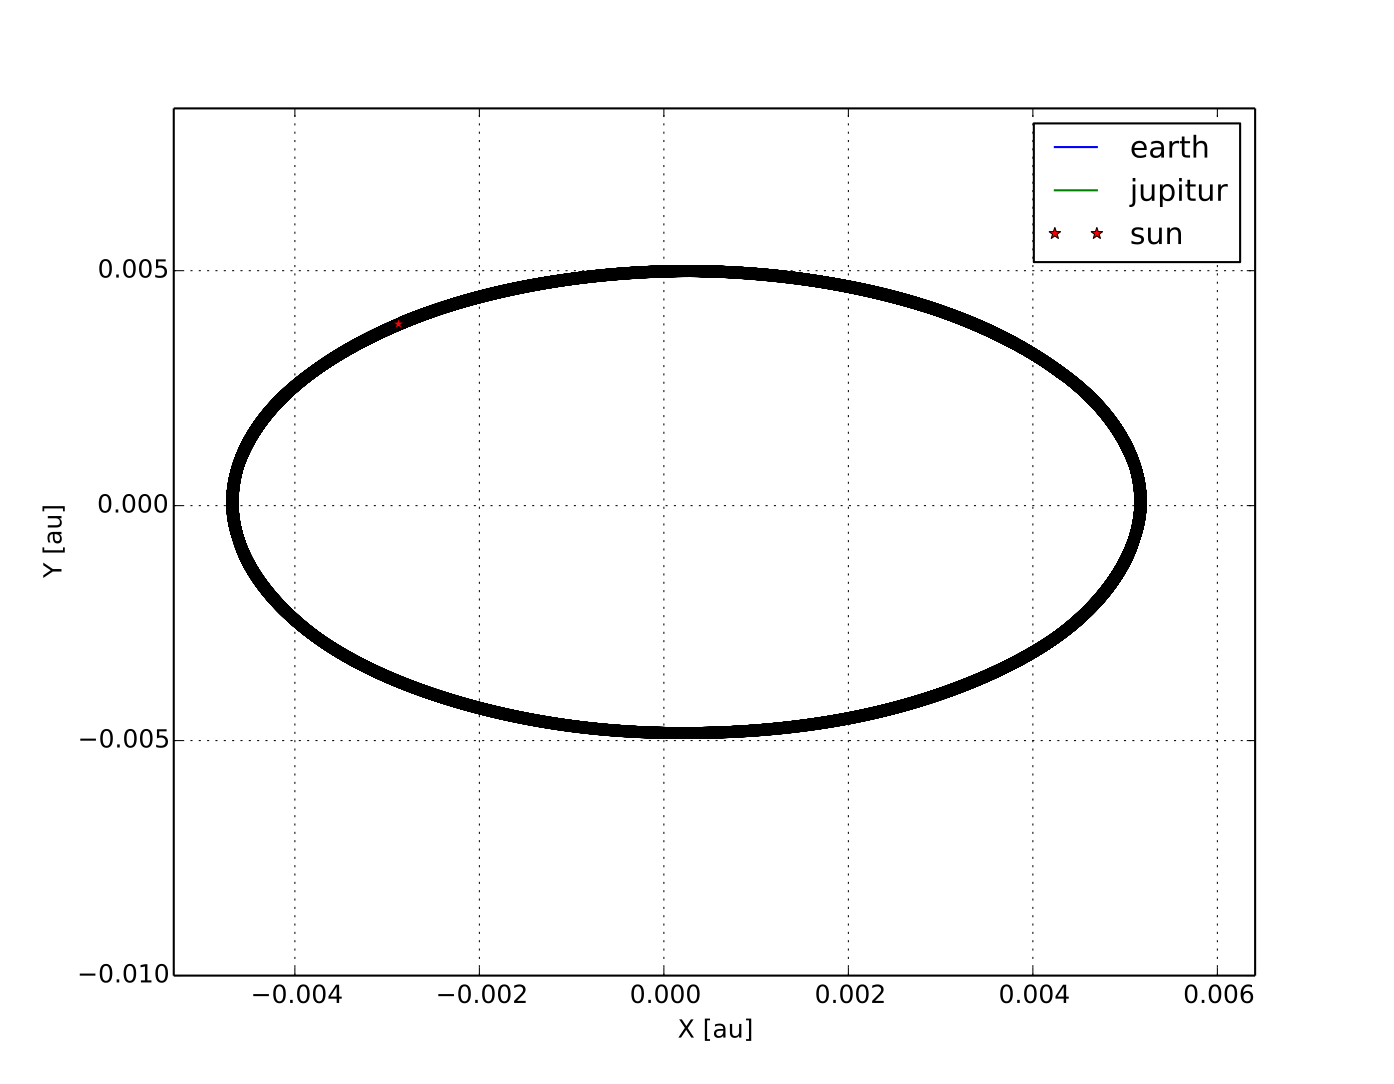
\includegraphics[width=\linewidth]{result/bilder/all-moving-jupitur-mass-center.png}
        \caption{}
    \end{subfigure}
    \caption{ n=$10^5$ and ran for 15 years. a) Shows the three body system solved with a moving sun. I b) is a zoom of the middle part of a). This is for verifying that the sun moves around the center of mass and is not drifting.}
    \label{fig:three-body-moving}
\end{figure}

The figure above has n=$10^5$ and ran for 15 years. If this would be used for any tests I would recommend using more points. To use more points here would be stupid. You can't see the difference.

\subsubsection{Solar system all moving}

\begin{figure}[H]
    \centering
    \begin{subfigure}{0.5\textwidth}
        \centering
        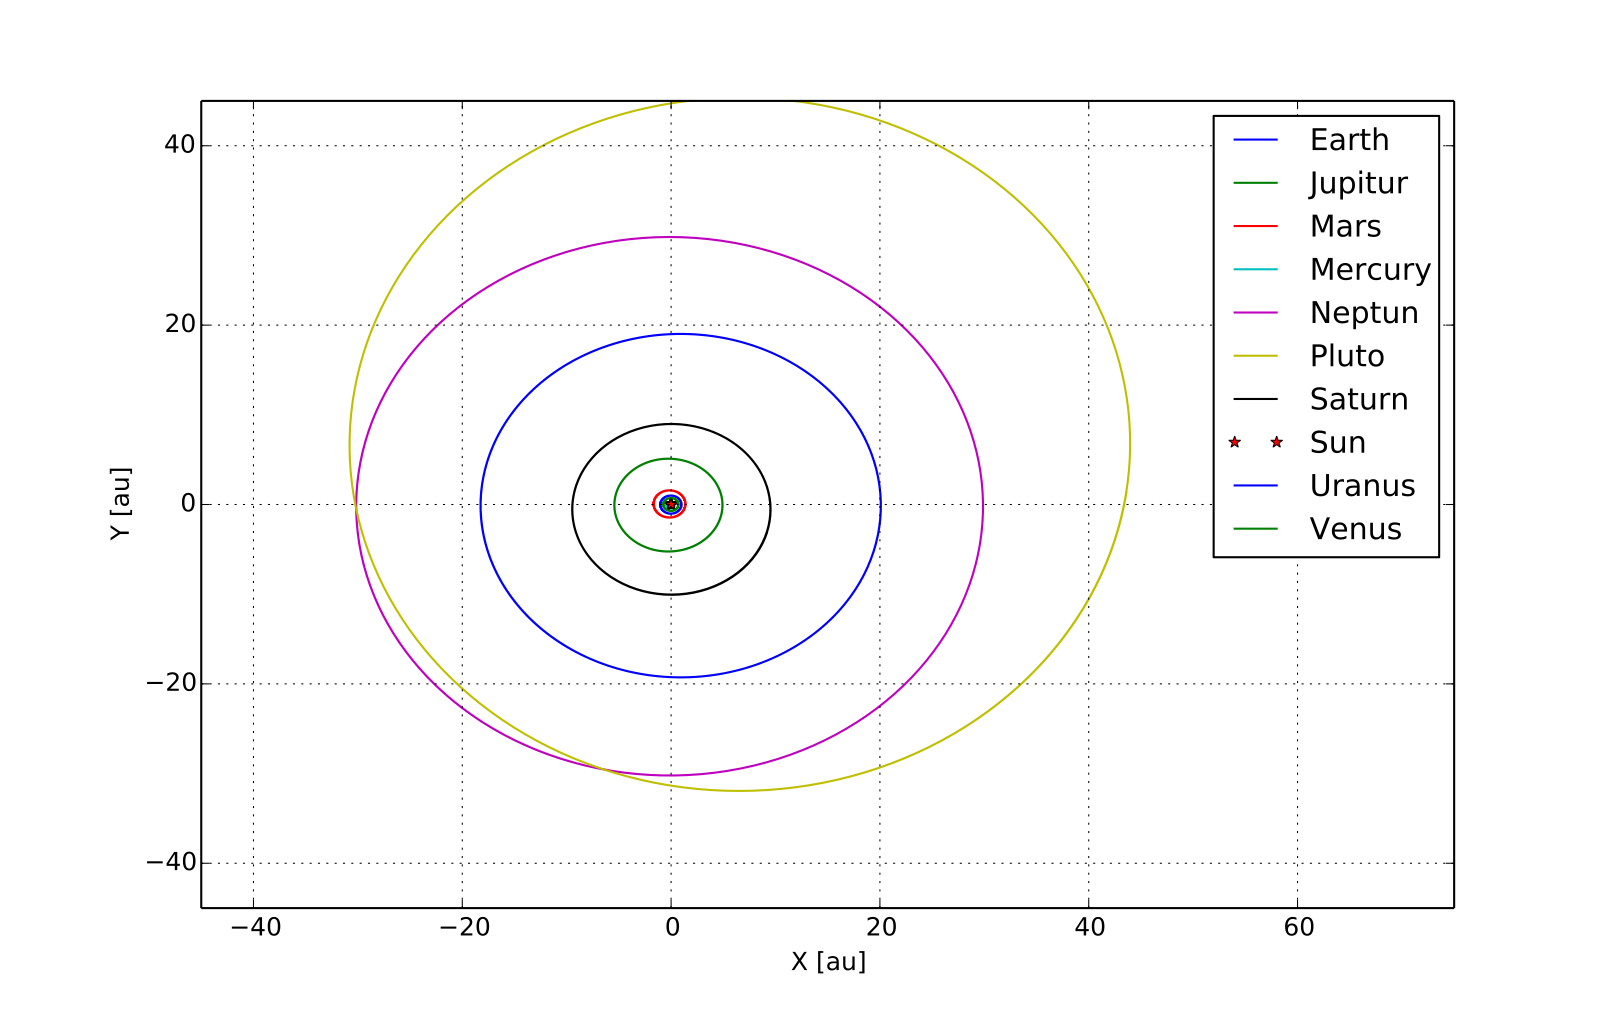
\includegraphics[width=\linewidth]{result/bilder/all-moving-solarsystem.png}
        \caption{}
    \end{subfigure}%
    ~ 
    \begin{subfigure}{0.5\textwidth}
        \centering
        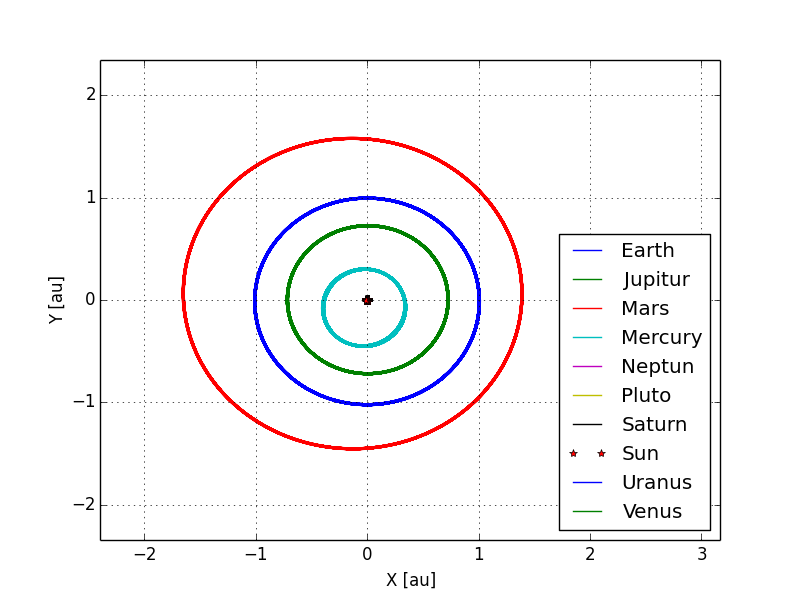
\includegraphics[width=\linewidth]{result/bilder/all-moving-solarsystem-zoom.png}
        \caption{}
    \end{subfigure}
    \caption{a) Shows the whole solar system solved with a moving sun.  b) is a zoom of the middle part of a). }
    \label{fig:solarsystem-moving}
\end{figure}

It has a n=$10^6$ and ran for 300 years. If this would be used for any tests I would recommend using more points, but this would be stupid for this figure, since you can't see the difference. Figure \ref{fig:solarsystem-moving} b) is for verifying that the sun also move in orbits around the center of mass, which is set to (0,0,0).


\pagebreak
\subsection{The perihelion precession of Mercury}

This has been discussed in section \ref{sec:perihelion}. The figure in this section was made from the results and python script in the directory \href{https://github.com/erikfsk/Project-3/tree/master/Project3/mercury-perihelion}{\textcolor{blue}{mercury-perihelion}}.


\begin{figure}[H]
    \centering
    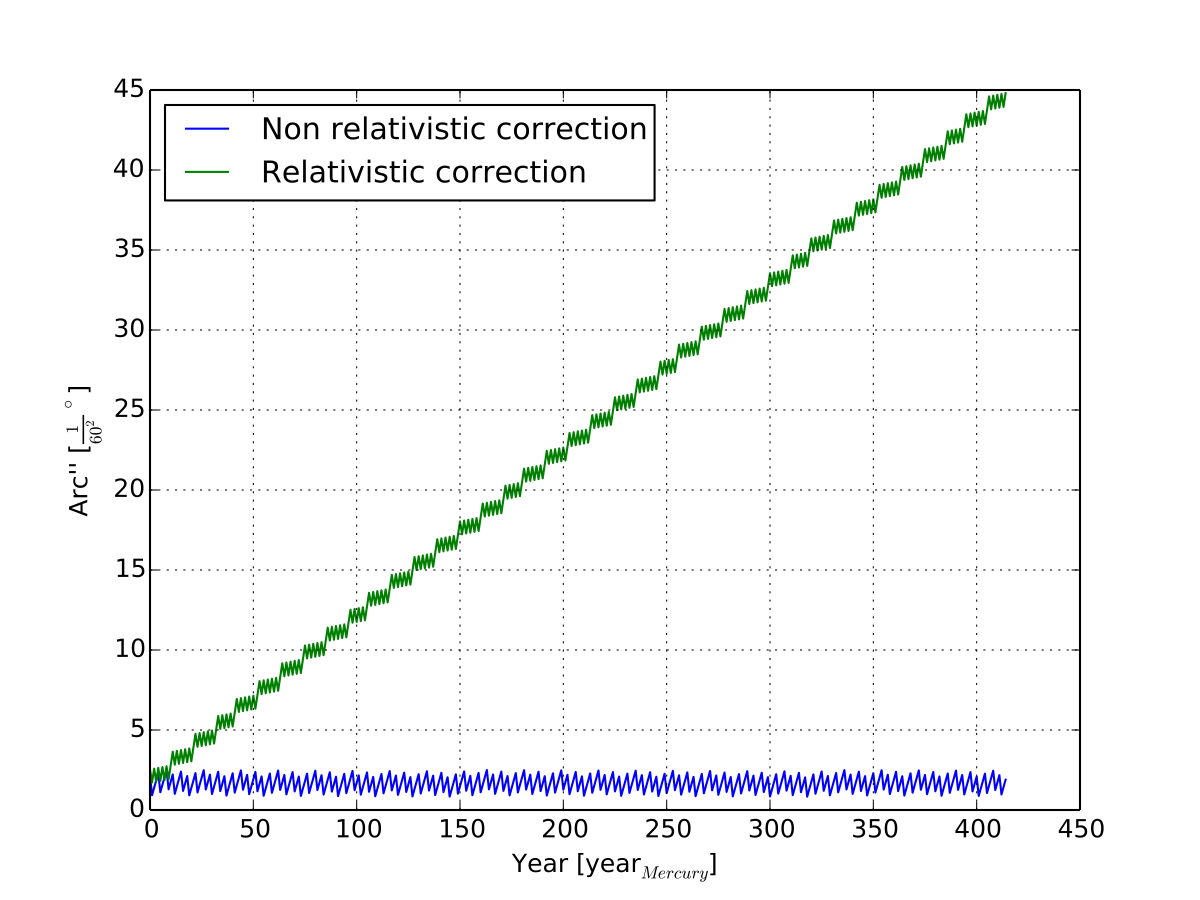
\includegraphics[width=0.8\linewidth]{result/bilder/perihelion.png}
    \caption{The graphs shows how Mercury orbit has moved in arc seconds as a function of orbits for Mercury.}
    \label{fig:perihelion}
\end{figure}

 After 100 years mercury perihelion should move about 43''. From the graphs we can see that it should move about 45''. This is probably due to numerical imprecision. The slopes inaccuracy is probably caused by the numerical solver precision. In other words more points would increase the accuracy. The jumping up and down along the linear curve is probably duo to the computer's accuracy with numbers. This will also improve by more steps, but one of them might stop to improve before the other.









%\pagebreak
%\section{Discussion}
%\input{discussion/discussion}


\section{Conclusion}
Both numerical methods has been tested and the Verlet-Velocity method comes out as the best. The time is nearly the same, but the Verlet-Velocity conserves energies, momentum and angular momentum for the earth-sun system. After these different scenarios has been studied with mostly expected results. The most unexpected result was with the three body system when Jupiter had the same mass as the sun. Here the Verlet-Velocity method struggle to produce reasonable results. The relativistic effect on mercury was studied and we are happy to report that our results correspond to observed values\cite{project3}.
\\
\\
Future work should aim to get an adaptive step size for the solver. This would probably help the three-body system. It would also be nice if a simple interface was developed, so we dont need to hard code each test. 



\pagebreak
\section{References}
\printbibliography


\pagebreak
\section{Appendix}\label{sec:appendix}
\begin{lstlisting}[language=c++]
//FLOPs FOR ACCELERATION
// 1 FLOP * 3 directions
dx = x1 - x2
// 3 FLOPs
r = sqrt(dx*dx + dy*dy + dz*dz)
// 7 FLOPs
a = - (Gconst*m*M/(r*r)) / (m*r)
// 2 FLOPs * 3 directions
a = a + a*(x1-x2);																	
//TOTAL FLOPs = 19 FLOPs 


//FLOPs FOR POSITION :: EULER
// 2 FLOPs * 3 directions
x = x + t_step*Vx															
//TOTAL FLOPs = 6 FLOPs 


//FLOPs FOR VELOCITY :: EULER
// 2 FLOPs * 3 directions
Vx = Vx + t_step*ax															
//TOTAL FLOPs = 6 FLOPs 


//FLOPs FOR POSITION :: Verlet
// 6 FLOPs * 3 directions
x = x + t_step*Vx + (0.5*t_step*t_step*a);
//TOTAL FLOPs = 21 FLOPs


//FLOPs FOR VELOCITY :: Verlet
// 4 FLOPs * 3 directions
Vx = Vx + (0.5*t_step*(Ax+Ax_old));
//TOTAL FLOPs = 12 FLOPs
\end{lstlisting}

\pagebreak

\begin{figure}[H]
		\centering
		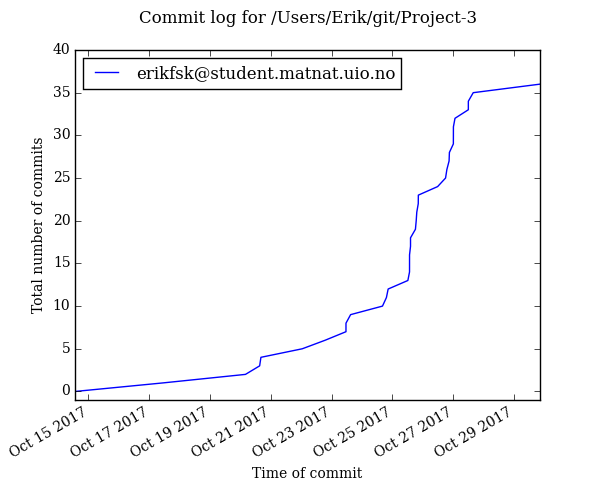
\includegraphics[width=0.7\linewidth]{appendix/bilder/workflow.png}
		\caption{Our retarded workflow... Next time maybe it will be better?}
		\label{fig:ab}
\end{figure}



%\begin{align*}
%&n \qquad &2^n - (-1)^n\\
%&n+1 \qquad &2^{n+1} - (-1)^{n+1} \\
%& &= 2(2^{n}) - (-1)^{n+1}\\
%& &= 2(2^{n} + (-1)^n  + (-1)^{n+1}) - (-1)^{n+1}\\
%& &= 2(2^{n} + (-1)^n  - (-1)^{n}) - (-1)^{n+1}\\
%& &= 2(2^{n}- (-1)^{n}) + 2(-1)^n  + (-1)^{n}\\
%& &= 2(2^{n}- (-1)^{n}) + 3(-1)^n \\
%\end{align*}



%\begin{tabular}{|c|c|c|c|c|c|c|}
%	\hline 
%	n & General & Specific & LU & fastest & slowest & $\frac{slowest}{fastest}$\\ 
%	\hline
%	10 & 6.5e-05 & 5e-06 & 4e-05 & Specific & General & 13.0\\ 
%	\hline 
%	100 & 7.5e-05 & 8e-06 & 0.0023 & Specific & LU & 287.5\\ 
%	\hline 
%	1000 & 0.00014 & 4e-05 & 0.26 & Specific & LU & 6500\\ 
%	\hline
%	10000 & 0.0007 & 0.0005 & 142.5 & Specific & LU & 285000 \\ 
%	\hline
%\end{tabular}

%\begin{figure}[H]
%		\centering
%		\includegraphics[width=0.7\linewidth]{ab.png}
%		\caption{Atomene er gule kuler, de elementære vektorene er blå og a vektorene er grønne.}
%		\label{fig:ab}
%\end{figure}



\end{document}
